\documentclass[compress]{beamer}
\usepackage[utf8]{inputenc}
%!TEX encoding = UTF-8 Unicode
\usepackage{amsmath}
\usepackage{amsfonts}
\usepackage{amssymb}
\usepackage[american]{babel}
\usepackage{xspace}
\usepackage{graphicx,psfrag}
\usepackage{CJK}
\usepackage{rotating}
\usepackage{pstool}
\usepackage{ifthen}
\usepackage{figlatex}


\graphicspath{{fig/}}


\mode<presentation>
{
  \usetheme{Replica}
  \setbeamercovered{transparent}
%  \setbeamertemplate{mini frames}[tick]
%  \setbeamertemplate{mini frame in other subsection}{}
}

\makeatletter
\let\beamer@writeslidentry@miniframeson=\beamer@writeslidentry
\def\beamer@writeslidentry@miniframesoff{%
  \expandafter\beamer@ifempty\expandafter{\beamer@framestartpage}{}% does not happen normally
  {%else
    % removed \addtocontents commands
    \clearpage\beamer@notesactions%
  }
}
\newcount\beamer@writeslidentry@miniframesoneoversome@counter
\newcount\beamer@writeslidentry@miniframesoneoversome@limit
\beamer@writeslidentry@miniframesoneoversome@counter=1
\newcount\beamer@writeslidentry@miniframesoneoversome@limit
\beamer@writeslidentry@miniframesoneoversome@limit=5
\def\beamer@writeslidentry@miniframesoneoversome{%
  \ifnum\beamer@writeslidentry@miniframesoneoversome@counter=\beamer@writeslidentry@miniframesoneoversome@limit\relax%
    \beamer@writeslidentry@miniframesoneoversome@counter=1\relax%
    \beamer@writeslidentry@miniframeson%
  \else%
    \advance\beamer@writeslidentry@miniframesoneoversome@counter by 1%
    \beamer@writeslidentry@miniframesoff%
  \fi%
}
\newcommand*{\miniframeson}{\let\beamer@writeslidentry=\beamer@writeslidentry@miniframeson}
\newcommand*{\miniframesoff}{\let\beamer@writeslidentry=\beamer@writeslidentry@miniframesoff}
\newcommand*{\miniframesalternate}[1]{%
   \beamer@writeslidentry@miniframesoneoversome@counter=1\relax%
   \beamer@writeslidentry@miniframesoneoversome@limit=#1\relax%
   \let\beamer@writeslidentry=\beamer@writeslidentry@miniframesoneoversome}

% Define the subsectionsonly option for beamer toc
\def\beamer@tocaction@only#1{\only<.(1)>{\usebeamertemplate**{#1}}}
\define@key{beamertoc}{subsectionsonly}[]{\beamer@toc@subsectionstyle{show/only}\beamer@toc@subsubsectionstyle{show/shaded/hide}}
\makeatother


\usepackage{relsize}
\usepackage{wasysym}
\def\smiley{\green{\larger[2]\wasyfamily\char44}\xspace}
\def\frownie{\blue{\larger[2]\wasyfamily\char47}\xspace}
\def\quesley{\yyellow{\hbox to -0.08em{\textraiseglotstop}$_{\textrm{\wasyfamily\char47}}$}\xspace}


%% Macros
\newcommand{\probaSymbol}{\mathbb P}
\newcommand{\proba}[1]{\probaSymbol\left(#1\right)}
\newcommand{\esperance}[1]{\mathbb E\left(#1\right)}
\newcommand{\Psachant} [2]{\mathbb P\left(#1\left|\,\vphantom{#1} #2\right.\right)} %proba de #1 sachant #2
\newcommand{\Esachant} [2]{\mathbb E\left(#1\left|\,\vphantom{#1} #2\right.\right)} %proba de #1 sachant #2


\newcommand<>{\blue}[1]{{\color#2{blue!100!black!100}#1}}
\newcommand<>{\redd}[1]{{\color#2{red!80!black}#1}}
\newcommand<>{\green}[1]{{\color#2{green!70!black}#1}}
\newcommand<>{\purple}[1]{{\color#2{blue!50!red}#1}}
\newcommand{\red}[1]{\textcolor{red}{#1}\xspace}
\title[Cooperative Checkpointing]{Optimal Cooperative Checkpointing for Shared High-Performance Computing Platforms}

\usepackage{xcolor,soul}
\sethlcolor{green}
\definecolor{cinnabar}{rgb}{1,0.5,0.5}
\makeatletter
\newcommand\SoulColor{%
  \let\set@color\beamerorig@set@color
  \let\reset@color\beamerorig@reset@color}
\makeatother
\usepackage[most]{tcolorbox}
\newtcolorbox{myblock}[2][]{beamer,title=#2,fonttitle=\sffamily,
  left=1mm,right=1mm,top=1mm,bottom=1mm,arc=2mm,
  colback=black,colupper=white,colframe=yellow,
  coltitle=black,title style={top color=red!70,bottom color=yellow},
  #1}

\usepackage{gnuplot-lua-tikz}
\newcommand{\muind}{\mu_{\text{ind}}}
\newcommand{\bandtotal}{\beta_{\text{tot}}}
\newcommand{\bandavail}{\beta_{\text{avail}}}
\newcommand{\appset}{{\mathcal A}}
\newcommand{\nbnodesplat}{{\mathcal N}}
\newcommand{\nbapps}{|{\mathcal A}|}
\newcommand{\app}[1]{A_{#1}}
\newcommand{\application}[2]{a_{#1}^{#2}}
\newcommand{\nbapp}[1]{n_{#1}}
\newcommand{\nbnodes}[1]{q_{#1}}
\newcommand{\period}[1]{P_{#1}}
\newcommand{\ckpt}[1]{C_{#1}}
\newcommand{\reco}[1]{R_{#1}}
\newcommand{\size}[1]{\mathit{size}_{#1}}
\newcommand{\wasteapp}[1]{W_{#1}}
\newcommand{\wap}[1]{W_{#1}}
\newcommand{\wapp}[2]{W_{#1}(#2)}
\newcommand{\mtbfplat}{\mu}
\newcommand{\wasteplat}{W}
\newcommand{\wasteplatt}{\textsc{Waste}\xspace}
\newcommand{\opt}{{\textit opt}}
\newcommand{\lost}{{\textit lost}}
\newcommand{\EE}{{\mathbb E}}
\newcommand{\ioconstraint}{F}
\newcommand{\lastckpt}[2]{L_{#1}^{#2}}
\newcommand{\wastefct}[2]{W_{#1}(#2)}
\newcommand{\pool}{{\mathcal P}}
\newcommand{\risk}{{\textsc Risk}}
%\newcommand{\todo}[1]{\textit{TBD: [#1]}}
\newcommand{\dca}[1]{\todo[inline]{DCA: #1}}
\newcommand{\kbf}[1]{\todo[inline]{kbf: #1}}

\newcommand{\IOcat}{\textsc{IO-Candidate}\xspace}
\newcommand{\Ckptcat}{\textsc{Ckpt-Candidate}\xspace}
\newcommand{\Catiocat}{\mathcal{C}_{IO}\xspace}
\newcommand{\Catckptcat}{\mathcal{C}_{Ckpt}\xspace}

\newcommand{\nocoop}{\emph{Oblivious}\xspace}
\newcommand{\fifoblock}{\emph{Ordered}\xspace}
\newcommand{\fifononblock}{\emph{Ordered-NB}\xspace}
\newcommand{\leastwaste}{\emph{Least-Waste}\xspace}

\def\propfixed{\nocoop-Fixed\xspace}
\def\propdaly{\nocoop-Daly\xspace}
\def\bfifofixed{\fifoblock-Fixed\xspace}
\def\bfifodaly{\fifoblock-Daly\xspace}
\def\fifofixed{\fifononblock-Fixed\xspace}
\def\fifodaly{\fifononblock-Daly\xspace}
\def\cooperative{\leastwaste}



\subtitle{}

\author[yves.robert@inria.fr]{%
\includegraphics[width=1cm,height=1.26cm]{photos/thomas.jpg}
\includegraphics[width=1cm,height=1.26cm]{photos/clooney.jpg}
\includegraphics[width=1cm,height=1.26cm]{photos/aurelien.jpg}
\includegraphics[width=1cm,height=1.26cm]{photos/dorian.jpg}
\includegraphics[width=1cm,height=1.26cm]{photos/kurt.jpg}
\includegraphics[width=1cm,height=1.26cm]{photos/george.jpg}
\includegraphics[width=1cm,height=1.26cm]{photos/jack.jpg}\\
~\\
{\footnotesize
Thomas Herault$^{1}$,
\textcolor{red}{Yves Robert}$^{1,2}$ 
Aurélien Bouteiller$^{1}$,\\
Dorian Arnold$^{3}$,
Kurt Ferreira$^{4}$,
George Bosilca$^{1}$,
Jack Dongarra$^{1}$\\
}
{\tiny
~\\
1. University of Tennessee Knoxville, USA\\
2. Laboratoire LIP, ENS Lyon \& Inria, France\\
3. Emory University, Atlanta, GA, USA\\
4. Sandia National Laboratory, USA\\
}}


\date[April 17, 2018]{\textcolor{green}{8th JLESC Workshop -- Barcelona -- April 17, 2018}}

\AtBeginSection[]
{
  \begin{frame}<beamer>
    \frametitle{Outline}
     {\scriptsize
       \tableofcontents[sectionstyle=show/shaded,subsectionstyle=show/show/hide]
    }
  \end{frame}
}

\AtBeginSubsection[]
{
  \begin{frame}<beamer>
    \frametitle{Outline}
     {\scriptsize
       \tableofcontents[sectionstyle=show/shaded,subsectionstyle=show/shaded/hide]
    }
  \end{frame}
}

\begin{document}

\miniframesalternate{5}
\pgfaliasimage{figbackground}{figbackground-orange}% !!!

\begin{frame}
  \titlepage
\end{frame}


\begin{frame}
  \frametitle{Framework}

\begin{itemize}
\item \green{Space-sharing} prevalent in HPC platforms
\item Application instances:
\begin{itemize}
\item have dedicated computational nodes
\item share interconnect links and storage partition (PFS)
\item checkpoint (to stable storage) independently
\end{itemize}
$\Rightarrow$ \redd{network and storage contention}
\end{itemize}

\end{frame}

\section{Problem Statement}

\begin{frame}
    \frametitle{Checkpointing 101}


\begin{center}
\includegraphics[width=11cm]{photos/faults.png}
\end{center}

\vfill
\noindent
\textbf{When do applications checkpoint on HPC systems?}
\begin{itemize}
\item Standard practice:  every hour 
\item State-of-the-art: Young/Daly period
\end{itemize}

\end{frame}

\begin{frame}
    \frametitle{Optimal checkpointing period}

\begin{center}
%\vspace{-2.5mm}
\includegraphics[width=0.8\textwidth]{photos/resilience.jpg}
\end{center}

\end{frame}

\begin{frame}
    \frametitle{Optimal checkpointing period}

\noindent
With period $T$:

\vfill
$$\wasteplatt \approx \frac{C}{T} + \frac{1}{\mu} \frac{T}{2} =
\frac{C}{T} + \frac{N}{\mu_{ind}}\frac{T}{2}$$

\vfill
$$\redd{T_{\opt} = \sqrt{2 C \mu} = \sqrt{\frac{2 C \mu_{ind}}{N}}} \qquad \green{\text{(Young/Daly)}}$$
$$\wasteplatt_{\opt} = \frac{2C}{\mu} = \frac{2CN}{\mu_{ind}}$$

\end{frame}

\begin{frame}
  \frametitle{How long does it take to checkpoint?}

\begin{center}
\vspace{-0.7cm}
\includegraphics[width=0.8\textwidth]{photos/Interference.pdf}
\end{center}

\vspace{-1.5cm}
\begin{itemize}
\item Optimal period computed assuming fixed checkpoint cost

\item Interferences between checkpointing I/O of App 1 and App 2 change their
checkpoint time\\
$\Rightarrow$ Applications checkpoint too often\\
%$\qquad\Rightarrow$ No optimal period any longer
\end{itemize}

\vfill
\textcolor{red}{When to checkpoint} in a shared environment,\\
$\qquad$ since \textcolor{red}{checkpoint cost is not predictible}?

\end{frame}

\section{Model}

\begin{frame}
  \frametitle{Model}

\noindent
\textbf{Platform}
\begin{itemize}
\item I/O subsystem time-shared (contended) 
\item Linear interference model
\end{itemize}

\noindent
\textbf{Workload}
\begin{itemize}
\item Many applications but only a few classes (sets of applications with similar sizes, durations, footprints and I/O needs)
\item Initialization and finalization I/O at max bandwidth;\\
regular (non-CR) I/O evenly distributed over execution
\item Job makespans known a priori
\item Simulations based on APEX workflow / Cielo platform
\end{itemize}

\noindent
\textbf{Checkpoint}
\begin{itemize}
\item Fixed: 1 hour (unless otherwise specified)
\item Daly:  uses  Young/Daly application period $\sqrt{2 C_{app} \mu_{app}}$
\end{itemize}

\end{frame}

\begin{frame}
  \frametitle{Notations}


\begin{itemize}
\item Set $\appset$ of applications classes
$\app{1}, \ldots \app{\nbapps}$
\item Platform with
$\nbnodesplat$ nodes
\item Application class $\app{i}$ specifies
\begin{itemize}
\item $\nbapp{i}$: number of jobs in $\app{i}$;
\item $\nbnodes{i}$: number of nodes used by each job in $\app{i}$;
\item $\period{i}$: checkpoint period of each job in $\app{i}$
\item $\ckpt{i}$ and $\reco{i}$: checkpoint and recovery for each job in $\app{i}$\\
(when no interference with other I/O operations)
\item Jobs inherit their characteristics from their classes
\item $\period{Daly}(J_{j}) = \sqrt{2 \ckpt{j} \mu_{j}}$, where
$\mu_{j} = \frac{\muind}{\nbnodes{j}}$ 
\end{itemize}
\end{itemize}
\end{frame}

\section{I/O Scheduling Algorithms}

\begin{frame}
  \frametitle{I/O Scheduling Algorithms}

%  \noindent\begin{tabular}{p{.5\linewidth}p{.5\linewidth}}
             \textbf{\nocoop (\textcolor[rgb]{0.86,0.39,0.21}{Fixed} / \textcolor[rgb]{0.93,0.73,0.27}{Daly})}\par
             {\small No scheduling of any I/O: when overlapping, interfere
             linearly}\par
             {\scriptsize $\Rightarrow$ Risk of \textcolor{red}{I/O Inefficiency}}

%             & 

               \textbf{\fifoblock (\textcolor[rgb]{0.17,0.38,0.15}{Fixed} / \textcolor[rgb]{0.46,0.67,0.19}{Daly})}\par
               {\small I/O (checkpoint or init/final) served First Come -
               First Served\\
               If another application is being served,
               wait in turn}\par
               {\scriptsize $\Rightarrow$ Risk of \textcolor{red}{delayed I/O} and
               checkpoints, increasing waste}

%               \\
             \textbf{\fifononblock (\textcolor[rgb]{0,0.44,0.74}{Fixed} / \textcolor[rgb]{0.33,0.75,0.93}{Daly})}\par
             {\small I/O (checkpoint or init/final) served First Come -
               First Served\\
               In case of checkpoints, continue
             working until served}\par
             {\scriptsize $\Rightarrow$ Risk of \textcolor{red}{over re-execution}
             due to delayed checkpoints}

%             &

               \textbf{\textcolor[rgb]{0.57,0.22,0.56}{\leastwaste}}\par
               {\small Serve I/O request that minimizes potential waste\par}
               {\scriptsize$\Rightarrow$ Checkpoints are \textcolor{blue}{non-blocking}: continue
               working until they are served\par
               $\Rightarrow$ \textcolor{blue}{Daly period} embedded in
               scheduling (prevent from checkpointing too often}
%               \\
%  \end{tabular}

\end{frame}

\begin{frame}
  \frametitle{\nocoop }


\begin{itemize}
\item Jobs fill up the system based on
processor availability
\item I/O workloads (including CR activities) \redd{not} coordinated
\item Each I/O stream given decrease in bandwidth linearly
proportional to the number of competing operations
\item  Subsequent checkpoint scheduled to start after
$\period{i}-\ckpt{i}$\\
$\Rightarrow$  Resultant checkpoint period may be longer than $\period{i}$

\end{itemize}

\end{frame}

\begin{frame}
  \frametitle{\fifoblock}


\begin{itemize}
\item Blocking FCFS I/O Scheduling
\item I/O requests performed sequentially, in request arrival order
\item Jobs
with outstanding I/O requests blocked until their requests are completed
\item  With  two jobs simultaneously requesting I/O of volume $V_1, V_2$:
\begin{itemize}
\item \nocoop:  Linear interference (both jobs I/O are slowed down)
  until the smallest of $(V_1, V_2)$ is transferred
\item \fifoblock:\\
- first scheduled job
takes $\frac{V_1}{\bandavail}$\\
- second job waits
$\frac{V_1}{\bandavail}$ then takes $\frac{V_2}{\bandavail}$
\end{itemize}
\item Resultant checkpoint period may be longer than $\period{i}$
\end{itemize}
\end{frame}

\begin{frame}
  \frametitle{\fifononblock}


\begin{itemize}
\item Non-Blocking FCFS I/O Scheduling
\item Refactor code to continue computing while awaiting
\textbf{checkpoint} I/O
\item  Previous
checkpoint ends at time $t_{now}$\\
$\Rightarrow$ tentative time for next checkpoint $t_{req}=t_{now}+\period{i}-\ckpt{i}$
\item At $t_{req}$, make non-blocking I/O request (I/O token still FCFS)
\item Job continues until I/O token is available
\item At this point, job generates its checkpoint data
\item Use existing APIs in SCR or FTI to regularly poll if a
checkpoint should be taken at this time
\item \redd{Postponed checkpoint $\Rightarrow$  increased risk exposure}
\end{itemize}

\end{frame}

%\begin{frame}
%  \frametitle{Variants}
%
%
%\begin{itemize}
%\item $\period{i}$ input parameter to \nocoop, \fifoblock and \fifononblock
%\item  Use either Fixed or Daly in simulations
%\end{itemize}
%
%\end{frame}

 \begin{frame}
  \frametitle{ \leastwaste}


\begin{itemize}
\item Non-Blocking \green{least waste} I/O Scheduling
\item When an I/O request completes at time $t$,\\
select best candidate from pool:
\begin{itemize}
\item \IOcat $\Catiocat$\\
   Job $J_{i}$, $1\leq i \leq r$ with an
  (input, output or recovery) I/O request of length $v_{i}$ seconds, has $q_{i}$
  processors, initiated its I/O request $d_{i}$ seconds ago (idle since)
\item \Ckptcat $\Catckptcat$\\
Job $J_{i}$, $r+1\leq i \leq r+s$,
  with a checkpoint duration of $C_{i}$ seconds and $q_{i}$ processors,
   took its last checkpoint $d_{i}$ seconds ago and keeps executing, with
  $d_{i} \geq \period{Daly}(J_{i})$
\end{itemize}

\end{itemize}

\end{frame}

 \begin{frame}
  \frametitle{Job selection}


\begin{itemize}

\item $J_{i} \in \Catiocat$  uses the I/O resource for $v_{i}$ seconds
\begin{itemize}
\item For $J_{j} \in \Catiocat$,  $\wapp{i}{j} = q_{j} (d_{j} + v_{i})$ 
\item For $J_{j} \in \Catckptcat$, $\wapp{i}{j} =
  \frac{v_{i}}{\muind} q^{2}_{j} (\reco{j} + d_{j} + \frac{v_{i}}{2})$
 \item Expected waste $\wap{i} = \sum_{J_{j} \in \Catiocat, j\neq i} \wapp{i}{j} + \sum_{J_{j} \in \Catckptcat} \wapp{i}{j}$
 \end{itemize}
 
 \item $J_{i} \in \Catckptcat$ uses  the I/O resource for $\ckpt{i}$ seconds
 \begin{itemize}
\item Similar equations \dots
  \end{itemize}
\item  Select job $J_{i} \in \Catiocat \cup \Catckptcat$
whose waste $\wap{i}$ is minimal
 
 \end{itemize}



\end{frame}


 \begin{frame}
  \frametitle{Feasibility of Cooperative Strategies}


\begin{itemize}
\item \fifoblock, \fifononblock, 
\leastwaste \redd{require synchronization}
\item \fifoblock\\
at filesystem level
\item  \fifononblock and
\leastwaste:\\
modify apps to continue working until access is granted\\
$\Rightarrow$ implementation in checkpointing library SCR or FTI
\item Memory
hierarchy:\\
- checkpoint process memory on unreliable (but
fast) media\\
- upload checkpoints in the background,\\
while the application proceeds to compute

 \end{itemize}

\end{frame}

\section{Lower bound}


 \begin{frame}
  \frametitle{Steady-state}
  
  
 \begin{itemize}
\item$\nbapp{i}$ jobs of class $\app{i}$, $\nbnodes{i}$ nodes, $\ckpt{i} =
\frac{\size{i}}{\bandavail}$
\item Waste  of $J_{i}$  with checkpoint period $\period{i}$:
$$\wasteapp{i} = \wastefct{i}{\period{i}} = \frac{\ckpt{i}}{\period{i}} +
\frac{\nbnodes{i}}{\mtbfplat}(\frac{\period{i}}{2} + \reco{i})$$
 \end{itemize}
 
 
\vfill
\noindent
\textsc{Minimize} 
$$\wasteplat = \sum_i \frac{\nbapp{i} \nbnodes{i}}{\nbnodesplat}  \left( \frac{\ckpt{i}}{\period{i}} +
\frac{\nbnodes{i}}{\mtbfplat}(\frac{\period{i}}{2} + \reco{i}) \right)$$

\noindent
\textsc{Subject to} 
$$\ioconstraint = \sum_{i} \frac{\nbapp{i} \ckpt{i}}{\period{i}} \leq 1$$


\end{frame}

 \begin{frame}
  \frametitle{Lower bound}


\noindent
\textsc{KKT} 
$$\period{i} = \sqrt{\frac{2 \mtbfplat  \nbnodesplat}{\nbnodes{i}^{2}} \left(\frac{\nbnodes{i}}{\nbnodesplat} +\lambda \right) \ckpt{i}}$$

\vfill
\begin{itemize}
\item Choose $\lambda$ minimal s.t. $\ioconstraint \leq 1$ (solve numerically)
\item $\lambda=0$ $\Rightarrow$ Young/Daly
\item I/O constraint not sufficient\\
$\Rightarrow$ orchestrate checkpoints into periodic repeating pattern\\
$\Rightarrow$ lower bound of $\wasteplat = \sum_i \frac{\nbapp{i} \nbnodes{i}}{\nbnodesplat} \wasteapp{i}(\period{i})$

 \end{itemize}

\end{frame}


\section{Simulations}


 \begin{frame}
  \frametitle{Simulation Framework}

\begin{itemize}
\item Random selection of jobs according to class ratios
\item Duration uniformly distributed between $0.8w$ and $1.2w$
\item Generation of node failures with Exponential distributions
\item First-fit strategy (job characteristics, job priority, 
resource availability)
\item Simulate online scheduling

\item Restarted jobs set to highest
priority


\end{itemize}


\end{frame}

\begin{frame}
  \frametitle{LANL Workloads from the APEX Workflows report}
  
\begin{center}
   
  
   {\scriptsize
\begin{tabular}{|l|c|c|c|c|}
\hline
 Workflow & EAP & LAP & Silverton & VPIC \\\hline
Workload percentage & 66 & 5.5 & 16.5 & 12 \\\hline
Work time (h) & 262.4 & 64 & 128 & 157.2 \\\hline
Number of cores & 16384 & 4096 & 32768 & 30000 \\\hline
Initial Input (\% of memory) &  3 & 5 & 70 & 10 \\\hline
Final Output (\% of memory) & 105 & 220 & 43 & 270 \\\hline
Checkpoint Size (\% of memory) & 160 & 185 & 350 & 85 \\\hline
\end{tabular}
}
 \end{center}

\vfill
\noindent
\textbf{Cielo} 
\begin{itemize}
\item
1.37 Petaflops capability system at LANL (2010-2016)
\item143,104 cores, 286 TB main memory
\item PFS with theoretical maximum capacity 160GB/s
\end{itemize}
\end{frame}


\begin{frame}
  \frametitle{Slowdown of checkpoints}
 
  \begin{center}
    \resizebox{0.95\linewidth}{!}{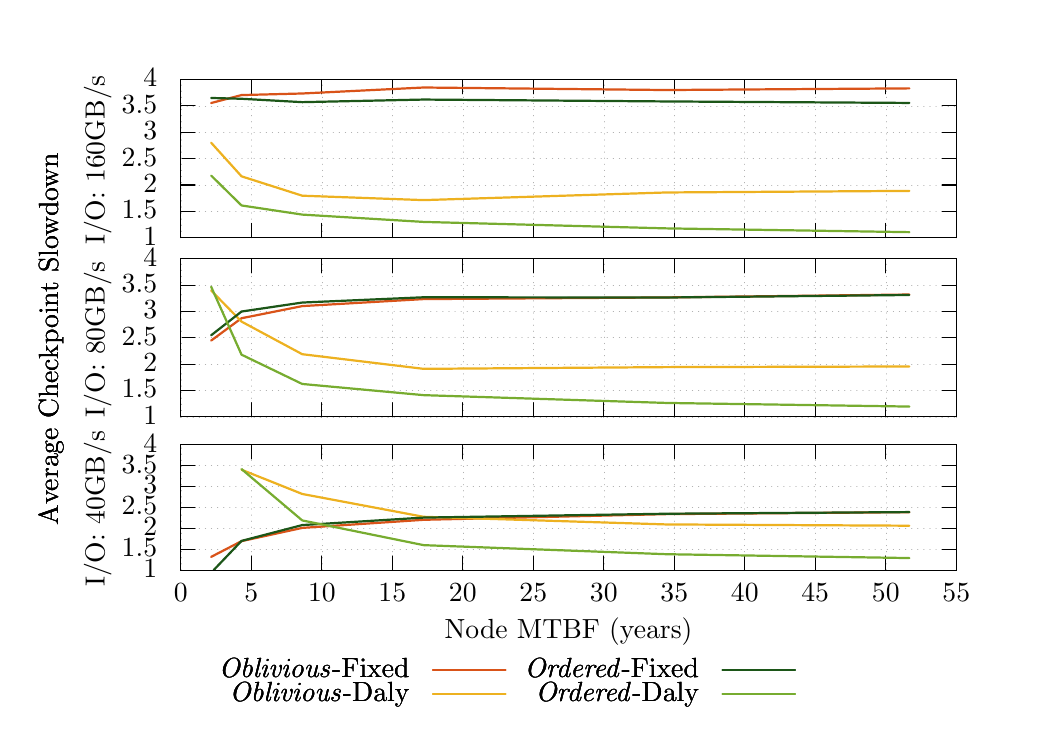
\begin{tikzpicture}[gnuplot]
%% generated with GNUPLOT 5.2p2 (Lua 5.3; terminal rev. 99, script rev. 102)
%% Tue Jan 30 12:37:29 2018
\path (0.000,0.000) rectangle (12.500,8.750);
\gpcolor{color=gp lt color axes}
\gpsetlinetype{gp lt axes}
\gpsetdashtype{gp dt axes}
\gpsetlinewidth{0.50}
\draw[gp path] (1.945,1.860)--(11.793,1.860);
\gpcolor{color=gp lt color border}
\gpsetlinetype{gp lt border}
\gpsetdashtype{gp dt solid}
\gpsetlinewidth{1.00}
\draw[gp path] (1.945,1.860)--(2.125,1.860);
\draw[gp path] (11.793,1.860)--(11.613,1.860);
\node[gp node right] at (1.761,1.860) {$1$};
\gpcolor{color=gp lt color axes}
\gpsetlinetype{gp lt axes}
\gpsetdashtype{gp dt axes}
\gpsetlinewidth{0.50}
\draw[gp path] (1.945,2.126)--(11.793,2.126);
\gpcolor{color=gp lt color border}
\gpsetlinetype{gp lt border}
\gpsetdashtype{gp dt solid}
\gpsetlinewidth{1.00}
\draw[gp path] (1.945,2.126)--(2.125,2.126);
\draw[gp path] (11.793,2.126)--(11.613,2.126);
\node[gp node right] at (1.761,2.126) {$1.5$};
\gpcolor{color=gp lt color axes}
\gpsetlinetype{gp lt axes}
\gpsetdashtype{gp dt axes}
\gpsetlinewidth{0.50}
\draw[gp path] (1.945,2.391)--(11.793,2.391);
\gpcolor{color=gp lt color border}
\gpsetlinetype{gp lt border}
\gpsetdashtype{gp dt solid}
\gpsetlinewidth{1.00}
\draw[gp path] (1.945,2.391)--(2.125,2.391);
\draw[gp path] (11.793,2.391)--(11.613,2.391);
\node[gp node right] at (1.761,2.391) {$2$};
\gpcolor{color=gp lt color axes}
\gpsetlinetype{gp lt axes}
\gpsetdashtype{gp dt axes}
\gpsetlinewidth{0.50}
\draw[gp path] (1.945,2.657)--(11.793,2.657);
\gpcolor{color=gp lt color border}
\gpsetlinetype{gp lt border}
\gpsetdashtype{gp dt solid}
\gpsetlinewidth{1.00}
\draw[gp path] (1.945,2.657)--(2.125,2.657);
\draw[gp path] (11.793,2.657)--(11.613,2.657);
\node[gp node right] at (1.761,2.657) {$2.5$};
\gpcolor{color=gp lt color axes}
\gpsetlinetype{gp lt axes}
\gpsetdashtype{gp dt axes}
\gpsetlinewidth{0.50}
\draw[gp path] (1.945,2.923)--(11.793,2.923);
\gpcolor{color=gp lt color border}
\gpsetlinetype{gp lt border}
\gpsetdashtype{gp dt solid}
\gpsetlinewidth{1.00}
\draw[gp path] (1.945,2.923)--(2.125,2.923);
\draw[gp path] (11.793,2.923)--(11.613,2.923);
\node[gp node right] at (1.761,2.923) {$3$};
\gpcolor{color=gp lt color axes}
\gpsetlinetype{gp lt axes}
\gpsetdashtype{gp dt axes}
\gpsetlinewidth{0.50}
\draw[gp path] (1.945,3.188)--(11.793,3.188);
\gpcolor{color=gp lt color border}
\gpsetlinetype{gp lt border}
\gpsetdashtype{gp dt solid}
\gpsetlinewidth{1.00}
\draw[gp path] (1.945,3.188)--(2.125,3.188);
\draw[gp path] (11.793,3.188)--(11.613,3.188);
\node[gp node right] at (1.761,3.188) {$3.5$};
\gpcolor{color=gp lt color axes}
\gpsetlinetype{gp lt axes}
\gpsetdashtype{gp dt axes}
\gpsetlinewidth{0.50}
\draw[gp path] (1.945,3.454)--(11.793,3.454);
\gpcolor{color=gp lt color border}
\gpsetlinetype{gp lt border}
\gpsetdashtype{gp dt solid}
\gpsetlinewidth{1.00}
\draw[gp path] (1.945,3.454)--(2.125,3.454);
\draw[gp path] (11.793,3.454)--(11.613,3.454);
\node[gp node right] at (1.761,3.454) {$4$};
\gpcolor{color=gp lt color axes}
\gpsetlinetype{gp lt axes}
\gpsetdashtype{gp dt axes}
\gpsetlinewidth{0.50}
\draw[gp path] (1.945,1.860)--(1.945,3.454);
\gpcolor{color=gp lt color border}
\gpsetlinetype{gp lt border}
\gpsetdashtype{gp dt solid}
\gpsetlinewidth{1.00}
\draw[gp path] (1.945,1.860)--(1.945,2.040);
\draw[gp path] (1.945,3.454)--(1.945,3.274);
\node[gp node center] at (1.945,1.552) {$0$};
\gpcolor{color=gp lt color axes}
\gpsetlinetype{gp lt axes}
\gpsetdashtype{gp dt axes}
\gpsetlinewidth{0.50}
\draw[gp path] (2.840,1.860)--(2.840,3.454);
\gpcolor{color=gp lt color border}
\gpsetlinetype{gp lt border}
\gpsetdashtype{gp dt solid}
\gpsetlinewidth{1.00}
\draw[gp path] (2.840,1.860)--(2.840,2.040);
\draw[gp path] (2.840,3.454)--(2.840,3.274);
\node[gp node center] at (2.840,1.552) {$5$};
\gpcolor{color=gp lt color axes}
\gpsetlinetype{gp lt axes}
\gpsetdashtype{gp dt axes}
\gpsetlinewidth{0.50}
\draw[gp path] (3.736,1.860)--(3.736,3.454);
\gpcolor{color=gp lt color border}
\gpsetlinetype{gp lt border}
\gpsetdashtype{gp dt solid}
\gpsetlinewidth{1.00}
\draw[gp path] (3.736,1.860)--(3.736,2.040);
\draw[gp path] (3.736,3.454)--(3.736,3.274);
\node[gp node center] at (3.736,1.552) {$10$};
\gpcolor{color=gp lt color axes}
\gpsetlinetype{gp lt axes}
\gpsetdashtype{gp dt axes}
\gpsetlinewidth{0.50}
\draw[gp path] (4.631,1.860)--(4.631,3.454);
\gpcolor{color=gp lt color border}
\gpsetlinetype{gp lt border}
\gpsetdashtype{gp dt solid}
\gpsetlinewidth{1.00}
\draw[gp path] (4.631,1.860)--(4.631,2.040);
\draw[gp path] (4.631,3.454)--(4.631,3.274);
\node[gp node center] at (4.631,1.552) {$15$};
\gpcolor{color=gp lt color axes}
\gpsetlinetype{gp lt axes}
\gpsetdashtype{gp dt axes}
\gpsetlinewidth{0.50}
\draw[gp path] (5.526,1.860)--(5.526,3.454);
\gpcolor{color=gp lt color border}
\gpsetlinetype{gp lt border}
\gpsetdashtype{gp dt solid}
\gpsetlinewidth{1.00}
\draw[gp path] (5.526,1.860)--(5.526,2.040);
\draw[gp path] (5.526,3.454)--(5.526,3.274);
\node[gp node center] at (5.526,1.552) {$20$};
\gpcolor{color=gp lt color axes}
\gpsetlinetype{gp lt axes}
\gpsetdashtype{gp dt axes}
\gpsetlinewidth{0.50}
\draw[gp path] (6.421,1.860)--(6.421,3.454);
\gpcolor{color=gp lt color border}
\gpsetlinetype{gp lt border}
\gpsetdashtype{gp dt solid}
\gpsetlinewidth{1.00}
\draw[gp path] (6.421,1.860)--(6.421,2.040);
\draw[gp path] (6.421,3.454)--(6.421,3.274);
\node[gp node center] at (6.421,1.552) {$25$};
\gpcolor{color=gp lt color axes}
\gpsetlinetype{gp lt axes}
\gpsetdashtype{gp dt axes}
\gpsetlinewidth{0.50}
\draw[gp path] (7.317,1.860)--(7.317,3.454);
\gpcolor{color=gp lt color border}
\gpsetlinetype{gp lt border}
\gpsetdashtype{gp dt solid}
\gpsetlinewidth{1.00}
\draw[gp path] (7.317,1.860)--(7.317,2.040);
\draw[gp path] (7.317,3.454)--(7.317,3.274);
\node[gp node center] at (7.317,1.552) {$30$};
\gpcolor{color=gp lt color axes}
\gpsetlinetype{gp lt axes}
\gpsetdashtype{gp dt axes}
\gpsetlinewidth{0.50}
\draw[gp path] (8.212,1.860)--(8.212,3.454);
\gpcolor{color=gp lt color border}
\gpsetlinetype{gp lt border}
\gpsetdashtype{gp dt solid}
\gpsetlinewidth{1.00}
\draw[gp path] (8.212,1.860)--(8.212,2.040);
\draw[gp path] (8.212,3.454)--(8.212,3.274);
\node[gp node center] at (8.212,1.552) {$35$};
\gpcolor{color=gp lt color axes}
\gpsetlinetype{gp lt axes}
\gpsetdashtype{gp dt axes}
\gpsetlinewidth{0.50}
\draw[gp path] (9.107,1.860)--(9.107,3.454);
\gpcolor{color=gp lt color border}
\gpsetlinetype{gp lt border}
\gpsetdashtype{gp dt solid}
\gpsetlinewidth{1.00}
\draw[gp path] (9.107,1.860)--(9.107,2.040);
\draw[gp path] (9.107,3.454)--(9.107,3.274);
\node[gp node center] at (9.107,1.552) {$40$};
\gpcolor{color=gp lt color axes}
\gpsetlinetype{gp lt axes}
\gpsetdashtype{gp dt axes}
\gpsetlinewidth{0.50}
\draw[gp path] (10.002,1.860)--(10.002,3.454);
\gpcolor{color=gp lt color border}
\gpsetlinetype{gp lt border}
\gpsetdashtype{gp dt solid}
\gpsetlinewidth{1.00}
\draw[gp path] (10.002,1.860)--(10.002,2.040);
\draw[gp path] (10.002,3.454)--(10.002,3.274);
\node[gp node center] at (10.002,1.552) {$45$};
\gpcolor{color=gp lt color axes}
\gpsetlinetype{gp lt axes}
\gpsetdashtype{gp dt axes}
\gpsetlinewidth{0.50}
\draw[gp path] (10.898,1.860)--(10.898,3.454);
\gpcolor{color=gp lt color border}
\gpsetlinetype{gp lt border}
\gpsetdashtype{gp dt solid}
\gpsetlinewidth{1.00}
\draw[gp path] (10.898,1.860)--(10.898,2.040);
\draw[gp path] (10.898,3.454)--(10.898,3.274);
\node[gp node center] at (10.898,1.552) {$50$};
\gpcolor{color=gp lt color axes}
\gpsetlinetype{gp lt axes}
\gpsetdashtype{gp dt axes}
\gpsetlinewidth{0.50}
\draw[gp path] (11.793,1.860)--(11.793,3.454);
\gpcolor{color=gp lt color border}
\gpsetlinetype{gp lt border}
\gpsetdashtype{gp dt solid}
\gpsetlinewidth{1.00}
\draw[gp path] (11.793,1.860)--(11.793,2.040);
\draw[gp path] (11.793,3.454)--(11.793,3.274);
\node[gp node center] at (11.793,1.552) {$55$};
\draw[gp path] (1.945,3.454)--(1.945,1.860)--(11.793,1.860)--(11.793,3.454)--cycle;
\node[gp node center,rotate=90] at (0.312,4.812) {Average Checkpoint Slowdown};
\node[gp node center,rotate=-270] at (0.901,2.657) {I/O: 40GB/s};
\node[gp node center] at (6.869,1.090) {Node MTBF (years)};
\node[gp node right] at (4.966,0.591) {\propfixed};
\gpcolor{rgb color={0.851,0.325,0.098}}
\gpsetlinewidth{2.00}
\draw[gp path] (5.150,0.591)--(6.066,0.591);
\draw[gp path] (2.330,2.029)--(2.716,2.229)--(3.487,2.397)--(5.029,2.500)--(8.113,2.572)%
  --(11.197,2.597);
\gpcolor{color=gp lt color border}
\node[gp node right] at (4.966,0.283) {\propdaly};
\gpcolor{rgb color={0.929,0.694,0.125}}
\draw[gp path] (5.150,0.283)--(6.066,0.283);
\draw[gp path] (2.716,3.136)--(3.487,2.828)--(5.029,2.538)--(8.113,2.441)--(11.197,2.425);
\gpcolor{color=gp lt color border}
\node[gp node right] at (8.642,0.591) {\bfifofixed};
\gpcolor{rgb color={0.110,0.337,0.094}}
\draw[gp path] (8.826,0.591)--(9.742,0.591);
\draw[gp path] (2.361,1.860)--(2.716,2.232)--(3.487,2.433)--(5.029,2.528)--(8.113,2.577)%
  --(11.197,2.598);
\gpcolor{color=gp lt color border}
\node[gp node right] at (8.642,0.283) {\bfifodaly};
\gpcolor{rgb color={0.467,0.675,0.188}}
\draw[gp path] (8.826,0.283)--(9.742,0.283);
\draw[gp path] (2.716,3.144)--(3.487,2.492)--(5.029,2.178)--(8.113,2.063)--(11.197,2.014);
\gpcolor{color=gp lt color border}
\gpsetlinewidth{1.00}
\draw[gp path] (1.945,3.454)--(1.945,1.860)--(11.793,1.860)--(11.793,3.454)--cycle;
%% coordinates of the plot area
\gpdefrectangularnode{gp plot 1}{\pgfpoint{1.945cm}{1.860cm}}{\pgfpoint{11.793cm}{3.454cm}}
\gpcolor{color=gp lt color axes}
\gpsetlinetype{gp lt axes}
\gpsetdashtype{gp dt axes}
\gpsetlinewidth{0.50}
\draw[gp path] (1.945,3.808)--(11.793,3.808);
\gpcolor{color=gp lt color border}
\gpsetlinetype{gp lt border}
\gpsetdashtype{gp dt solid}
\gpsetlinewidth{1.00}
\draw[gp path] (1.945,3.808)--(2.125,3.808);
\draw[gp path] (11.793,3.808)--(11.613,3.808);
\node[gp node right] at (1.761,3.808) {$1$};
\gpcolor{color=gp lt color axes}
\gpsetlinetype{gp lt axes}
\gpsetdashtype{gp dt axes}
\gpsetlinewidth{0.50}
\draw[gp path] (1.945,4.143)--(11.793,4.143);
\gpcolor{color=gp lt color border}
\gpsetlinetype{gp lt border}
\gpsetdashtype{gp dt solid}
\gpsetlinewidth{1.00}
\draw[gp path] (1.945,4.143)--(2.125,4.143);
\draw[gp path] (11.793,4.143)--(11.613,4.143);
\node[gp node right] at (1.761,4.143) {$1.5$};
\gpcolor{color=gp lt color axes}
\gpsetlinetype{gp lt axes}
\gpsetdashtype{gp dt axes}
\gpsetlinewidth{0.50}
\draw[gp path] (1.945,4.477)--(11.793,4.477);
\gpcolor{color=gp lt color border}
\gpsetlinetype{gp lt border}
\gpsetdashtype{gp dt solid}
\gpsetlinewidth{1.00}
\draw[gp path] (1.945,4.477)--(2.125,4.477);
\draw[gp path] (11.793,4.477)--(11.613,4.477);
\node[gp node right] at (1.761,4.477) {$2$};
\gpcolor{color=gp lt color axes}
\gpsetlinetype{gp lt axes}
\gpsetdashtype{gp dt axes}
\gpsetlinewidth{0.50}
\draw[gp path] (1.945,4.812)--(11.793,4.812);
\gpcolor{color=gp lt color border}
\gpsetlinetype{gp lt border}
\gpsetdashtype{gp dt solid}
\gpsetlinewidth{1.00}
\draw[gp path] (1.945,4.812)--(2.125,4.812);
\draw[gp path] (11.793,4.812)--(11.613,4.812);
\node[gp node right] at (1.761,4.812) {$2.5$};
\gpcolor{color=gp lt color axes}
\gpsetlinetype{gp lt axes}
\gpsetdashtype{gp dt axes}
\gpsetlinewidth{0.50}
\draw[gp path] (1.945,5.147)--(11.793,5.147);
\gpcolor{color=gp lt color border}
\gpsetlinetype{gp lt border}
\gpsetdashtype{gp dt solid}
\gpsetlinewidth{1.00}
\draw[gp path] (1.945,5.147)--(2.125,5.147);
\draw[gp path] (11.793,5.147)--(11.613,5.147);
\node[gp node right] at (1.761,5.147) {$3$};
\gpcolor{color=gp lt color axes}
\gpsetlinetype{gp lt axes}
\gpsetdashtype{gp dt axes}
\gpsetlinewidth{0.50}
\draw[gp path] (1.945,5.481)--(11.793,5.481);
\gpcolor{color=gp lt color border}
\gpsetlinetype{gp lt border}
\gpsetdashtype{gp dt solid}
\gpsetlinewidth{1.00}
\draw[gp path] (1.945,5.481)--(2.125,5.481);
\draw[gp path] (11.793,5.481)--(11.613,5.481);
\node[gp node right] at (1.761,5.481) {$3.5$};
\gpcolor{color=gp lt color axes}
\gpsetlinetype{gp lt axes}
\gpsetdashtype{gp dt axes}
\gpsetlinewidth{0.50}
\draw[gp path] (1.945,5.816)--(11.793,5.816);
\gpcolor{color=gp lt color border}
\gpsetlinetype{gp lt border}
\gpsetdashtype{gp dt solid}
\gpsetlinewidth{1.00}
\draw[gp path] (1.945,5.816)--(2.125,5.816);
\draw[gp path] (11.793,5.816)--(11.613,5.816);
\node[gp node right] at (1.761,5.816) {$4$};
\gpcolor{color=gp lt color axes}
\gpsetlinetype{gp lt axes}
\gpsetdashtype{gp dt axes}
\gpsetlinewidth{0.50}
\draw[gp path] (1.945,3.808)--(1.945,5.816);
\gpcolor{color=gp lt color border}
\gpsetlinetype{gp lt border}
\gpsetdashtype{gp dt solid}
\gpsetlinewidth{1.00}
\draw[gp path] (1.945,3.808)--(1.945,3.988);
\draw[gp path] (1.945,5.816)--(1.945,5.636);
\gpcolor{color=gp lt color axes}
\gpsetlinetype{gp lt axes}
\gpsetdashtype{gp dt axes}
\gpsetlinewidth{0.50}
\draw[gp path] (2.840,3.808)--(2.840,5.816);
\gpcolor{color=gp lt color border}
\gpsetlinetype{gp lt border}
\gpsetdashtype{gp dt solid}
\gpsetlinewidth{1.00}
\draw[gp path] (2.840,3.808)--(2.840,3.988);
\draw[gp path] (2.840,5.816)--(2.840,5.636);
\gpcolor{color=gp lt color axes}
\gpsetlinetype{gp lt axes}
\gpsetdashtype{gp dt axes}
\gpsetlinewidth{0.50}
\draw[gp path] (3.736,3.808)--(3.736,5.816);
\gpcolor{color=gp lt color border}
\gpsetlinetype{gp lt border}
\gpsetdashtype{gp dt solid}
\gpsetlinewidth{1.00}
\draw[gp path] (3.736,3.808)--(3.736,3.988);
\draw[gp path] (3.736,5.816)--(3.736,5.636);
\gpcolor{color=gp lt color axes}
\gpsetlinetype{gp lt axes}
\gpsetdashtype{gp dt axes}
\gpsetlinewidth{0.50}
\draw[gp path] (4.631,3.808)--(4.631,5.816);
\gpcolor{color=gp lt color border}
\gpsetlinetype{gp lt border}
\gpsetdashtype{gp dt solid}
\gpsetlinewidth{1.00}
\draw[gp path] (4.631,3.808)--(4.631,3.988);
\draw[gp path] (4.631,5.816)--(4.631,5.636);
\gpcolor{color=gp lt color axes}
\gpsetlinetype{gp lt axes}
\gpsetdashtype{gp dt axes}
\gpsetlinewidth{0.50}
\draw[gp path] (5.526,3.808)--(5.526,5.816);
\gpcolor{color=gp lt color border}
\gpsetlinetype{gp lt border}
\gpsetdashtype{gp dt solid}
\gpsetlinewidth{1.00}
\draw[gp path] (5.526,3.808)--(5.526,3.988);
\draw[gp path] (5.526,5.816)--(5.526,5.636);
\gpcolor{color=gp lt color axes}
\gpsetlinetype{gp lt axes}
\gpsetdashtype{gp dt axes}
\gpsetlinewidth{0.50}
\draw[gp path] (6.421,3.808)--(6.421,5.816);
\gpcolor{color=gp lt color border}
\gpsetlinetype{gp lt border}
\gpsetdashtype{gp dt solid}
\gpsetlinewidth{1.00}
\draw[gp path] (6.421,3.808)--(6.421,3.988);
\draw[gp path] (6.421,5.816)--(6.421,5.636);
\gpcolor{color=gp lt color axes}
\gpsetlinetype{gp lt axes}
\gpsetdashtype{gp dt axes}
\gpsetlinewidth{0.50}
\draw[gp path] (7.317,3.808)--(7.317,5.816);
\gpcolor{color=gp lt color border}
\gpsetlinetype{gp lt border}
\gpsetdashtype{gp dt solid}
\gpsetlinewidth{1.00}
\draw[gp path] (7.317,3.808)--(7.317,3.988);
\draw[gp path] (7.317,5.816)--(7.317,5.636);
\gpcolor{color=gp lt color axes}
\gpsetlinetype{gp lt axes}
\gpsetdashtype{gp dt axes}
\gpsetlinewidth{0.50}
\draw[gp path] (8.212,3.808)--(8.212,5.816);
\gpcolor{color=gp lt color border}
\gpsetlinetype{gp lt border}
\gpsetdashtype{gp dt solid}
\gpsetlinewidth{1.00}
\draw[gp path] (8.212,3.808)--(8.212,3.988);
\draw[gp path] (8.212,5.816)--(8.212,5.636);
\gpcolor{color=gp lt color axes}
\gpsetlinetype{gp lt axes}
\gpsetdashtype{gp dt axes}
\gpsetlinewidth{0.50}
\draw[gp path] (9.107,3.808)--(9.107,5.816);
\gpcolor{color=gp lt color border}
\gpsetlinetype{gp lt border}
\gpsetdashtype{gp dt solid}
\gpsetlinewidth{1.00}
\draw[gp path] (9.107,3.808)--(9.107,3.988);
\draw[gp path] (9.107,5.816)--(9.107,5.636);
\gpcolor{color=gp lt color axes}
\gpsetlinetype{gp lt axes}
\gpsetdashtype{gp dt axes}
\gpsetlinewidth{0.50}
\draw[gp path] (10.002,3.808)--(10.002,5.816);
\gpcolor{color=gp lt color border}
\gpsetlinetype{gp lt border}
\gpsetdashtype{gp dt solid}
\gpsetlinewidth{1.00}
\draw[gp path] (10.002,3.808)--(10.002,3.988);
\draw[gp path] (10.002,5.816)--(10.002,5.636);
\gpcolor{color=gp lt color axes}
\gpsetlinetype{gp lt axes}
\gpsetdashtype{gp dt axes}
\gpsetlinewidth{0.50}
\draw[gp path] (10.898,3.808)--(10.898,5.816);
\gpcolor{color=gp lt color border}
\gpsetlinetype{gp lt border}
\gpsetdashtype{gp dt solid}
\gpsetlinewidth{1.00}
\draw[gp path] (10.898,3.808)--(10.898,3.988);
\draw[gp path] (10.898,5.816)--(10.898,5.636);
\gpcolor{color=gp lt color axes}
\gpsetlinetype{gp lt axes}
\gpsetdashtype{gp dt axes}
\gpsetlinewidth{0.50}
\draw[gp path] (11.793,3.808)--(11.793,5.816);
\gpcolor{color=gp lt color border}
\gpsetlinetype{gp lt border}
\gpsetdashtype{gp dt solid}
\gpsetlinewidth{1.00}
\draw[gp path] (11.793,3.808)--(11.793,3.988);
\draw[gp path] (11.793,5.816)--(11.793,5.636);
\draw[gp path] (1.945,5.816)--(1.945,3.808)--(11.793,3.808)--(11.793,5.816)--cycle;
\node[gp node center,rotate=90] at (0.312,4.812) {Average Checkpoint Slowdown};
\node[gp node center,rotate=-270] at (0.901,4.812) {I/O: 80GB/s};
\node[gp node right] at (4.966,0.591) {\propfixed};
\gpcolor{rgb color={0.851,0.325,0.098}}
\gpsetlinewidth{2.00}
\draw[gp path] (5.150,0.591)--(6.066,0.591);
\draw[gp path] (2.330,4.776)--(2.716,5.060)--(3.487,5.214)--(5.029,5.303)--(8.113,5.324)%
  --(11.197,5.361);
\gpcolor{color=gp lt color border}
\node[gp node right] at (4.966,0.283) {\propdaly};
\gpcolor{rgb color={0.929,0.694,0.125}}
\draw[gp path] (5.150,0.283)--(6.066,0.283);
\draw[gp path] (2.330,5.412)--(2.716,5.017)--(3.487,4.603)--(5.029,4.417)--(8.113,4.439)%
  --(11.197,4.447);
\gpcolor{color=gp lt color border}
\node[gp node right] at (8.642,0.591) {\bfifofixed};
\gpcolor{rgb color={0.110,0.337,0.094}}
\draw[gp path] (8.826,0.591)--(9.742,0.591);
\draw[gp path] (2.330,4.843)--(2.716,5.145)--(3.487,5.259)--(5.029,5.326)--(8.113,5.323)%
  --(11.197,5.355);
\gpcolor{color=gp lt color border}
\node[gp node right] at (8.642,0.283) {\bfifodaly};
\gpcolor{rgb color={0.467,0.675,0.188}}
\draw[gp path] (8.826,0.283)--(9.742,0.283);
\draw[gp path] (2.330,5.460)--(2.716,4.597)--(3.487,4.225)--(5.029,4.083)--(8.113,3.984)%
  --(11.197,3.938);
\gpcolor{color=gp lt color border}
\gpsetlinewidth{1.00}
\draw[gp path] (1.945,5.816)--(1.945,3.808)--(11.793,3.808)--(11.793,5.816)--cycle;
%% coordinates of the plot area
\gpdefrectangularnode{gp plot 2}{\pgfpoint{1.945cm}{3.808cm}}{\pgfpoint{11.793cm}{5.816cm}}
\gpcolor{color=gp lt color axes}
\gpsetlinetype{gp lt axes}
\gpsetdashtype{gp dt axes}
\gpsetlinewidth{0.50}
\draw[gp path] (1.945,6.083)--(11.793,6.083);
\gpcolor{color=gp lt color border}
\gpsetlinetype{gp lt border}
\gpsetdashtype{gp dt solid}
\gpsetlinewidth{1.00}
\draw[gp path] (1.945,6.083)--(2.125,6.083);
\draw[gp path] (11.793,6.083)--(11.613,6.083);
\node[gp node right] at (1.761,6.083) {$1$};
\gpcolor{color=gp lt color axes}
\gpsetlinetype{gp lt axes}
\gpsetdashtype{gp dt axes}
\gpsetlinewidth{0.50}
\draw[gp path] (1.945,6.418)--(11.793,6.418);
\gpcolor{color=gp lt color border}
\gpsetlinetype{gp lt border}
\gpsetdashtype{gp dt solid}
\gpsetlinewidth{1.00}
\draw[gp path] (1.945,6.418)--(2.125,6.418);
\draw[gp path] (11.793,6.418)--(11.613,6.418);
\node[gp node right] at (1.761,6.418) {$1.5$};
\gpcolor{color=gp lt color axes}
\gpsetlinetype{gp lt axes}
\gpsetdashtype{gp dt axes}
\gpsetlinewidth{0.50}
\draw[gp path] (1.945,6.752)--(11.793,6.752);
\gpcolor{color=gp lt color border}
\gpsetlinetype{gp lt border}
\gpsetdashtype{gp dt solid}
\gpsetlinewidth{1.00}
\draw[gp path] (1.945,6.752)--(2.125,6.752);
\draw[gp path] (11.793,6.752)--(11.613,6.752);
\node[gp node right] at (1.761,6.752) {$2$};
\gpcolor{color=gp lt color axes}
\gpsetlinetype{gp lt axes}
\gpsetdashtype{gp dt axes}
\gpsetlinewidth{0.50}
\draw[gp path] (1.945,7.087)--(11.793,7.087);
\gpcolor{color=gp lt color border}
\gpsetlinetype{gp lt border}
\gpsetdashtype{gp dt solid}
\gpsetlinewidth{1.00}
\draw[gp path] (1.945,7.087)--(2.125,7.087);
\draw[gp path] (11.793,7.087)--(11.613,7.087);
\node[gp node right] at (1.761,7.087) {$2.5$};
\gpcolor{color=gp lt color axes}
\gpsetlinetype{gp lt axes}
\gpsetdashtype{gp dt axes}
\gpsetlinewidth{0.50}
\draw[gp path] (1.945,7.422)--(11.793,7.422);
\gpcolor{color=gp lt color border}
\gpsetlinetype{gp lt border}
\gpsetdashtype{gp dt solid}
\gpsetlinewidth{1.00}
\draw[gp path] (1.945,7.422)--(2.125,7.422);
\draw[gp path] (11.793,7.422)--(11.613,7.422);
\node[gp node right] at (1.761,7.422) {$3$};
\gpcolor{color=gp lt color axes}
\gpsetlinetype{gp lt axes}
\gpsetdashtype{gp dt axes}
\gpsetlinewidth{0.50}
\draw[gp path] (1.945,7.756)--(11.793,7.756);
\gpcolor{color=gp lt color border}
\gpsetlinetype{gp lt border}
\gpsetdashtype{gp dt solid}
\gpsetlinewidth{1.00}
\draw[gp path] (1.945,7.756)--(2.125,7.756);
\draw[gp path] (11.793,7.756)--(11.613,7.756);
\node[gp node right] at (1.761,7.756) {$3.5$};
\gpcolor{color=gp lt color axes}
\gpsetlinetype{gp lt axes}
\gpsetdashtype{gp dt axes}
\gpsetlinewidth{0.50}
\draw[gp path] (1.945,8.091)--(11.793,8.091);
\gpcolor{color=gp lt color border}
\gpsetlinetype{gp lt border}
\gpsetdashtype{gp dt solid}
\gpsetlinewidth{1.00}
\draw[gp path] (1.945,8.091)--(2.125,8.091);
\draw[gp path] (11.793,8.091)--(11.613,8.091);
\node[gp node right] at (1.761,8.091) {$4$};
\gpcolor{color=gp lt color axes}
\gpsetlinetype{gp lt axes}
\gpsetdashtype{gp dt axes}
\gpsetlinewidth{0.50}
\draw[gp path] (1.945,6.083)--(1.945,8.091);
\gpcolor{color=gp lt color border}
\gpsetlinetype{gp lt border}
\gpsetdashtype{gp dt solid}
\gpsetlinewidth{1.00}
\draw[gp path] (1.945,6.083)--(1.945,6.263);
\draw[gp path] (1.945,8.091)--(1.945,7.911);
\gpcolor{color=gp lt color axes}
\gpsetlinetype{gp lt axes}
\gpsetdashtype{gp dt axes}
\gpsetlinewidth{0.50}
\draw[gp path] (2.840,6.083)--(2.840,8.091);
\gpcolor{color=gp lt color border}
\gpsetlinetype{gp lt border}
\gpsetdashtype{gp dt solid}
\gpsetlinewidth{1.00}
\draw[gp path] (2.840,6.083)--(2.840,6.263);
\draw[gp path] (2.840,8.091)--(2.840,7.911);
\gpcolor{color=gp lt color axes}
\gpsetlinetype{gp lt axes}
\gpsetdashtype{gp dt axes}
\gpsetlinewidth{0.50}
\draw[gp path] (3.736,6.083)--(3.736,8.091);
\gpcolor{color=gp lt color border}
\gpsetlinetype{gp lt border}
\gpsetdashtype{gp dt solid}
\gpsetlinewidth{1.00}
\draw[gp path] (3.736,6.083)--(3.736,6.263);
\draw[gp path] (3.736,8.091)--(3.736,7.911);
\gpcolor{color=gp lt color axes}
\gpsetlinetype{gp lt axes}
\gpsetdashtype{gp dt axes}
\gpsetlinewidth{0.50}
\draw[gp path] (4.631,6.083)--(4.631,8.091);
\gpcolor{color=gp lt color border}
\gpsetlinetype{gp lt border}
\gpsetdashtype{gp dt solid}
\gpsetlinewidth{1.00}
\draw[gp path] (4.631,6.083)--(4.631,6.263);
\draw[gp path] (4.631,8.091)--(4.631,7.911);
\gpcolor{color=gp lt color axes}
\gpsetlinetype{gp lt axes}
\gpsetdashtype{gp dt axes}
\gpsetlinewidth{0.50}
\draw[gp path] (5.526,6.083)--(5.526,8.091);
\gpcolor{color=gp lt color border}
\gpsetlinetype{gp lt border}
\gpsetdashtype{gp dt solid}
\gpsetlinewidth{1.00}
\draw[gp path] (5.526,6.083)--(5.526,6.263);
\draw[gp path] (5.526,8.091)--(5.526,7.911);
\gpcolor{color=gp lt color axes}
\gpsetlinetype{gp lt axes}
\gpsetdashtype{gp dt axes}
\gpsetlinewidth{0.50}
\draw[gp path] (6.421,6.083)--(6.421,8.091);
\gpcolor{color=gp lt color border}
\gpsetlinetype{gp lt border}
\gpsetdashtype{gp dt solid}
\gpsetlinewidth{1.00}
\draw[gp path] (6.421,6.083)--(6.421,6.263);
\draw[gp path] (6.421,8.091)--(6.421,7.911);
\gpcolor{color=gp lt color axes}
\gpsetlinetype{gp lt axes}
\gpsetdashtype{gp dt axes}
\gpsetlinewidth{0.50}
\draw[gp path] (7.317,6.083)--(7.317,8.091);
\gpcolor{color=gp lt color border}
\gpsetlinetype{gp lt border}
\gpsetdashtype{gp dt solid}
\gpsetlinewidth{1.00}
\draw[gp path] (7.317,6.083)--(7.317,6.263);
\draw[gp path] (7.317,8.091)--(7.317,7.911);
\gpcolor{color=gp lt color axes}
\gpsetlinetype{gp lt axes}
\gpsetdashtype{gp dt axes}
\gpsetlinewidth{0.50}
\draw[gp path] (8.212,6.083)--(8.212,8.091);
\gpcolor{color=gp lt color border}
\gpsetlinetype{gp lt border}
\gpsetdashtype{gp dt solid}
\gpsetlinewidth{1.00}
\draw[gp path] (8.212,6.083)--(8.212,6.263);
\draw[gp path] (8.212,8.091)--(8.212,7.911);
\gpcolor{color=gp lt color axes}
\gpsetlinetype{gp lt axes}
\gpsetdashtype{gp dt axes}
\gpsetlinewidth{0.50}
\draw[gp path] (9.107,6.083)--(9.107,8.091);
\gpcolor{color=gp lt color border}
\gpsetlinetype{gp lt border}
\gpsetdashtype{gp dt solid}
\gpsetlinewidth{1.00}
\draw[gp path] (9.107,6.083)--(9.107,6.263);
\draw[gp path] (9.107,8.091)--(9.107,7.911);
\gpcolor{color=gp lt color axes}
\gpsetlinetype{gp lt axes}
\gpsetdashtype{gp dt axes}
\gpsetlinewidth{0.50}
\draw[gp path] (10.002,6.083)--(10.002,8.091);
\gpcolor{color=gp lt color border}
\gpsetlinetype{gp lt border}
\gpsetdashtype{gp dt solid}
\gpsetlinewidth{1.00}
\draw[gp path] (10.002,6.083)--(10.002,6.263);
\draw[gp path] (10.002,8.091)--(10.002,7.911);
\gpcolor{color=gp lt color axes}
\gpsetlinetype{gp lt axes}
\gpsetdashtype{gp dt axes}
\gpsetlinewidth{0.50}
\draw[gp path] (10.898,6.083)--(10.898,8.091);
\gpcolor{color=gp lt color border}
\gpsetlinetype{gp lt border}
\gpsetdashtype{gp dt solid}
\gpsetlinewidth{1.00}
\draw[gp path] (10.898,6.083)--(10.898,6.263);
\draw[gp path] (10.898,8.091)--(10.898,7.911);
\gpcolor{color=gp lt color axes}
\gpsetlinetype{gp lt axes}
\gpsetdashtype{gp dt axes}
\gpsetlinewidth{0.50}
\draw[gp path] (11.793,6.083)--(11.793,8.091);
\gpcolor{color=gp lt color border}
\gpsetlinetype{gp lt border}
\gpsetdashtype{gp dt solid}
\gpsetlinewidth{1.00}
\draw[gp path] (11.793,6.083)--(11.793,6.263);
\draw[gp path] (11.793,8.091)--(11.793,7.911);
\draw[gp path] (1.945,8.091)--(1.945,6.083)--(11.793,6.083)--(11.793,8.091)--cycle;
\node[gp node center,rotate=90] at (0.312,4.812) {Average Checkpoint Slowdown};
\node[gp node center,rotate=-270] at (0.901,7.087) {I/O: 160GB/s};
\node[gp node right] at (4.966,0.591) {\propfixed};
\gpcolor{rgb color={0.851,0.325,0.098}}
\gpsetlinewidth{2.00}
\draw[gp path] (5.150,0.591)--(6.066,0.591);
\draw[gp path] (2.330,7.793)--(2.716,7.894)--(3.487,7.914)--(5.029,7.990)--(8.113,7.958)%
  --(11.197,7.979);
\gpcolor{color=gp lt color border}
\node[gp node right] at (4.966,0.283) {\propdaly};
\gpcolor{rgb color={0.929,0.694,0.125}}
\draw[gp path] (5.150,0.283)--(6.066,0.283);
\draw[gp path] (2.330,7.289)--(2.716,6.862)--(3.487,6.616)--(5.029,6.560)--(8.113,6.657)%
  --(11.197,6.677);
\gpcolor{color=gp lt color border}
\node[gp node right] at (8.642,0.591) {\bfifofixed};
\gpcolor{rgb color={0.110,0.337,0.094}}
\draw[gp path] (8.826,0.591)--(9.742,0.591);
\draw[gp path] (2.330,7.857)--(2.716,7.847)--(3.487,7.804)--(5.029,7.837)--(8.113,7.813)%
  --(11.197,7.794);
\gpcolor{color=gp lt color border}
\node[gp node right] at (8.642,0.283) {\bfifodaly};
\gpcolor{rgb color={0.467,0.675,0.188}}
\draw[gp path] (8.826,0.283)--(9.742,0.283);
\draw[gp path] (2.330,6.872)--(2.716,6.492)--(3.487,6.376)--(5.029,6.283)--(8.113,6.201)%
  --(11.197,6.153);
\gpcolor{color=gp lt color border}
\gpsetlinewidth{1.00}
\draw[gp path] (1.945,8.091)--(1.945,6.083)--(11.793,6.083)--(11.793,8.091)--cycle;
%% coordinates of the plot area
\gpdefrectangularnode{gp plot 3}{\pgfpoint{1.945cm}{6.083cm}}{\pgfpoint{11.793cm}{8.091cm}}
\end{tikzpicture}
%% gnuplot variables
}
 \end{center}
      
      \end{frame}
      
      
      \begin{frame}
  \frametitle{Waste as a function of system bandwidth}
 
  \begin{center}
    \resizebox{0.95\linewidth}{!}{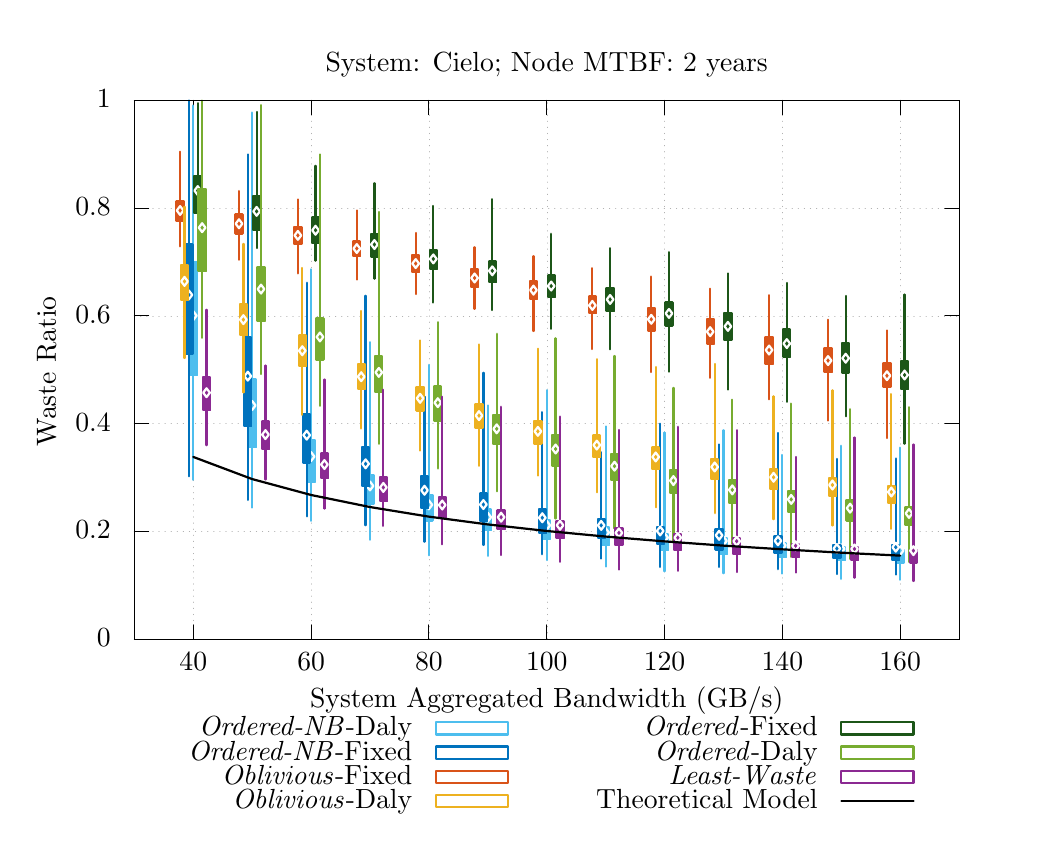
\begin{tikzpicture}[gnuplot]
%% generated with GNUPLOT 5.0p6 (Lua 5.3; terminal rev. 99, script rev. 100)
%% Thu Oct 19 13:54:21 2017
\path (0.000,0.000) rectangle (12.500,8.750);
\gpcolor{color=gp lt color axes}
\gpsetlinetype{gp lt axes}
\gpsetdashtype{gp dt axes}
\gpsetlinewidth{0.50}
\draw[gp path] (1.320,0.985)--(11.793,0.985);
\gpcolor{color=gp lt color border}
\gpsetlinetype{gp lt border}
\gpsetdashtype{gp dt solid}
\gpsetlinewidth{1.00}
\draw[gp path] (1.320,0.985)--(1.500,0.985);
\draw[gp path] (11.793,0.985)--(11.613,0.985);
\node[gp node right] at (1.136,0.985) {$0$};
\gpcolor{color=gp lt color axes}
\gpsetlinetype{gp lt axes}
\gpsetdashtype{gp dt axes}
\gpsetlinewidth{0.50}
\draw[gp path] (1.320,2.353)--(11.793,2.353);
\gpcolor{color=gp lt color border}
\gpsetlinetype{gp lt border}
\gpsetdashtype{gp dt solid}
\gpsetlinewidth{1.00}
\draw[gp path] (1.320,2.353)--(1.500,2.353);
\draw[gp path] (11.793,2.353)--(11.613,2.353);
\node[gp node right] at (1.136,2.353) {$0.2$};
\gpcolor{color=gp lt color axes}
\gpsetlinetype{gp lt axes}
\gpsetdashtype{gp dt axes}
\gpsetlinewidth{0.50}
\draw[gp path] (1.320,3.721)--(11.793,3.721);
\gpcolor{color=gp lt color border}
\gpsetlinetype{gp lt border}
\gpsetdashtype{gp dt solid}
\gpsetlinewidth{1.00}
\draw[gp path] (1.320,3.721)--(1.500,3.721);
\draw[gp path] (11.793,3.721)--(11.613,3.721);
\node[gp node right] at (1.136,3.721) {$0.4$};
\gpcolor{color=gp lt color axes}
\gpsetlinetype{gp lt axes}
\gpsetdashtype{gp dt axes}
\gpsetlinewidth{0.50}
\draw[gp path] (1.320,5.089)--(11.793,5.089);
\gpcolor{color=gp lt color border}
\gpsetlinetype{gp lt border}
\gpsetdashtype{gp dt solid}
\gpsetlinewidth{1.00}
\draw[gp path] (1.320,5.089)--(1.500,5.089);
\draw[gp path] (11.793,5.089)--(11.613,5.089);
\node[gp node right] at (1.136,5.089) {$0.6$};
\gpcolor{color=gp lt color axes}
\gpsetlinetype{gp lt axes}
\gpsetdashtype{gp dt axes}
\gpsetlinewidth{0.50}
\draw[gp path] (1.320,6.457)--(11.793,6.457);
\gpcolor{color=gp lt color border}
\gpsetlinetype{gp lt border}
\gpsetdashtype{gp dt solid}
\gpsetlinewidth{1.00}
\draw[gp path] (1.320,6.457)--(1.500,6.457);
\draw[gp path] (11.793,6.457)--(11.613,6.457);
\node[gp node right] at (1.136,6.457) {$0.8$};
\gpcolor{color=gp lt color axes}
\gpsetlinetype{gp lt axes}
\gpsetdashtype{gp dt axes}
\gpsetlinewidth{0.50}
\draw[gp path] (1.320,7.825)--(11.793,7.825);
\gpcolor{color=gp lt color border}
\gpsetlinetype{gp lt border}
\gpsetdashtype{gp dt solid}
\gpsetlinewidth{1.00}
\draw[gp path] (1.320,7.825)--(1.500,7.825);
\draw[gp path] (11.793,7.825)--(11.613,7.825);
\node[gp node right] at (1.136,7.825) {$1$};
\gpcolor{color=gp lt color axes}
\gpsetlinetype{gp lt axes}
\gpsetdashtype{gp dt axes}
\gpsetlinewidth{0.50}
\draw[gp path] (2.068,0.985)--(2.068,7.825);
\gpcolor{color=gp lt color border}
\gpsetlinetype{gp lt border}
\gpsetdashtype{gp dt solid}
\gpsetlinewidth{1.00}
\draw[gp path] (2.068,0.985)--(2.068,1.165);
\draw[gp path] (2.068,7.825)--(2.068,7.645);
\node[gp node center] at (2.068,0.677) {$40$};
\gpcolor{color=gp lt color axes}
\gpsetlinetype{gp lt axes}
\gpsetdashtype{gp dt axes}
\gpsetlinewidth{0.50}
\draw[gp path] (3.564,0.985)--(3.564,7.825);
\gpcolor{color=gp lt color border}
\gpsetlinetype{gp lt border}
\gpsetdashtype{gp dt solid}
\gpsetlinewidth{1.00}
\draw[gp path] (3.564,0.985)--(3.564,1.165);
\draw[gp path] (3.564,7.825)--(3.564,7.645);
\node[gp node center] at (3.564,0.677) {$60$};
\gpcolor{color=gp lt color axes}
\gpsetlinetype{gp lt axes}
\gpsetdashtype{gp dt axes}
\gpsetlinewidth{0.50}
\draw[gp path] (5.060,0.985)--(5.060,7.825);
\gpcolor{color=gp lt color border}
\gpsetlinetype{gp lt border}
\gpsetdashtype{gp dt solid}
\gpsetlinewidth{1.00}
\draw[gp path] (5.060,0.985)--(5.060,1.165);
\draw[gp path] (5.060,7.825)--(5.060,7.645);
\node[gp node center] at (5.060,0.677) {$80$};
\gpcolor{color=gp lt color axes}
\gpsetlinetype{gp lt axes}
\gpsetdashtype{gp dt axes}
\gpsetlinewidth{0.50}
\draw[gp path] (6.557,0.985)--(6.557,7.825);
\gpcolor{color=gp lt color border}
\gpsetlinetype{gp lt border}
\gpsetdashtype{gp dt solid}
\gpsetlinewidth{1.00}
\draw[gp path] (6.557,0.985)--(6.557,1.165);
\draw[gp path] (6.557,7.825)--(6.557,7.645);
\node[gp node center] at (6.557,0.677) {$100$};
\gpcolor{color=gp lt color axes}
\gpsetlinetype{gp lt axes}
\gpsetdashtype{gp dt axes}
\gpsetlinewidth{0.50}
\draw[gp path] (8.053,0.985)--(8.053,7.825);
\gpcolor{color=gp lt color border}
\gpsetlinetype{gp lt border}
\gpsetdashtype{gp dt solid}
\gpsetlinewidth{1.00}
\draw[gp path] (8.053,0.985)--(8.053,1.165);
\draw[gp path] (8.053,7.825)--(8.053,7.645);
\node[gp node center] at (8.053,0.677) {$120$};
\gpcolor{color=gp lt color axes}
\gpsetlinetype{gp lt axes}
\gpsetdashtype{gp dt axes}
\gpsetlinewidth{0.50}
\draw[gp path] (9.549,0.985)--(9.549,7.825);
\gpcolor{color=gp lt color border}
\gpsetlinetype{gp lt border}
\gpsetdashtype{gp dt solid}
\gpsetlinewidth{1.00}
\draw[gp path] (9.549,0.985)--(9.549,1.165);
\draw[gp path] (9.549,7.825)--(9.549,7.645);
\node[gp node center] at (9.549,0.677) {$140$};
\gpcolor{color=gp lt color axes}
\gpsetlinetype{gp lt axes}
\gpsetdashtype{gp dt axes}
\gpsetlinewidth{0.50}
\draw[gp path] (11.045,0.985)--(11.045,7.825);
\gpcolor{color=gp lt color border}
\gpsetlinetype{gp lt border}
\gpsetdashtype{gp dt solid}
\gpsetlinewidth{1.00}
\draw[gp path] (11.045,0.985)--(11.045,1.165);
\draw[gp path] (11.045,7.825)--(11.045,7.645);
\node[gp node center] at (11.045,0.677) {$160$};
\draw[gp path] (1.320,7.825)--(1.320,0.985)--(11.793,0.985)--(11.793,7.825)--cycle;
\node[gp node center,rotate=-270] at (0.246,4.405) {Waste Ratio};
\node[gp node center] at (6.556,0.215) {System Aggregated Bandwidth (GB/s)};
\node[gp node center] at (6.556,8.287) {System: Cielo; Node MTBF: 2 years};
\node[gp node right] at (4.966,-0.149) {\fifodaly};
\gpcolor{rgb color={0.302,0.745,0.933}}
\gpsetlinewidth{2.00}
\draw[gp path] (5.150,-0.226)--(6.066,-0.226)--(6.066,-0.072)--(5.150,-0.072)--cycle;
\gpfill{rgb color={0.302,0.745,0.933}} (2.023,4.342)--(2.113,4.342)--(2.113,5.777)--(2.023,5.777)--cycle;
\draw[gp path] (2.068,3.009)--(2.068,4.342);
\draw[gp path] (2.068,5.777)--(2.068,7.761);
\draw[gp path] (2.023,5.777)--(2.113,5.777)--(2.113,4.342)--(2.023,4.342)--cycle;
\gpfill{rgb color={0.302,0.745,0.933}} (2.771,3.427)--(2.861,3.427)--(2.861,4.281)--(2.771,4.281)--cycle;
\draw[gp path] (2.816,2.655)--(2.816,3.427);
\draw[gp path] (2.816,4.281)--(2.816,7.672);
\draw[gp path] (2.771,4.281)--(2.861,4.281)--(2.861,3.427)--(2.771,3.427)--cycle;
\gpfill{rgb color={0.302,0.745,0.933}} (3.519,2.985)--(3.609,2.985)--(3.609,3.514)--(3.519,3.514)--cycle;
\draw[gp path] (3.564,2.487)--(3.564,2.985);
\draw[gp path] (3.564,3.514)--(3.564,5.681);
\draw[gp path] (3.519,3.514)--(3.609,3.514)--(3.609,2.985)--(3.519,2.985)--cycle;
\gpfill{rgb color={0.302,0.745,0.933}} (4.267,2.696)--(4.357,2.696)--(4.357,3.073)--(4.267,3.073)--cycle;
\draw[gp path] (4.312,2.247)--(4.312,2.696);
\draw[gp path] (4.312,3.073)--(4.312,4.755);
\draw[gp path] (4.267,3.073)--(4.357,3.073)--(4.357,2.696)--(4.267,2.696)--cycle;
\gpfill{rgb color={0.302,0.745,0.933}} (5.015,2.491)--(5.105,2.491)--(5.105,2.819)--(5.015,2.819)--cycle;
\draw[gp path] (5.060,2.049)--(5.060,2.491);
\draw[gp path] (5.060,2.819)--(5.060,4.468);
\draw[gp path] (5.015,2.819)--(5.105,2.819)--(5.105,2.491)--(5.015,2.491)--cycle;
\gpfill{rgb color={0.302,0.745,0.933}} (5.763,2.372)--(5.853,2.372)--(5.853,2.631)--(5.763,2.631)--cycle;
\draw[gp path] (5.808,2.041)--(5.808,2.372);
\draw[gp path] (5.808,2.631)--(5.808,3.952);
\draw[gp path] (5.763,2.631)--(5.853,2.631)--(5.853,2.372)--(5.763,2.372)--cycle;
\gpfill{rgb color={0.302,0.745,0.933}} (6.512,2.260)--(6.602,2.260)--(6.602,2.501)--(6.512,2.501)--cycle;
\draw[gp path] (6.557,1.989)--(6.557,2.260);
\draw[gp path] (6.557,2.501)--(6.557,4.145);
\draw[gp path] (6.512,2.501)--(6.602,2.501)--(6.602,2.260)--(6.512,2.260)--cycle;
\gpfill{rgb color={0.302,0.745,0.933}} (7.260,2.175)--(7.350,2.175)--(7.350,2.406)--(7.260,2.406)--cycle;
\draw[gp path] (7.305,1.906)--(7.305,2.175);
\draw[gp path] (7.305,2.406)--(7.305,3.686);
\draw[gp path] (7.260,2.406)--(7.350,2.406)--(7.350,2.175)--(7.260,2.175)--cycle;
\gpfill{rgb color={0.302,0.745,0.933}} (8.008,2.117)--(8.098,2.117)--(8.098,2.319)--(8.008,2.319)--cycle;
\draw[gp path] (8.053,1.846)--(8.053,2.117);
\draw[gp path] (8.053,2.319)--(8.053,3.608);
\draw[gp path] (8.008,2.319)--(8.098,2.319)--(8.098,2.117)--(8.008,2.117)--cycle;
\gpfill{rgb color={0.302,0.745,0.933}} (8.756,2.068)--(8.846,2.068)--(8.846,2.265)--(8.756,2.265)--cycle;
\draw[gp path] (8.801,1.821)--(8.801,2.068);
\draw[gp path] (8.801,2.265)--(8.801,3.638);
\draw[gp path] (8.756,2.265)--(8.846,2.265)--(8.846,2.068)--(8.756,2.068)--cycle;
\gpfill{rgb color={0.302,0.745,0.933}} (9.504,2.026)--(9.594,2.026)--(9.594,2.199)--(9.504,2.199)--cycle;
\draw[gp path] (9.549,1.817)--(9.549,2.026);
\draw[gp path] (9.549,2.199)--(9.549,3.324);
\draw[gp path] (9.504,2.199)--(9.594,2.199)--(9.594,2.026)--(9.504,2.026)--cycle;
\gpfill{rgb color={0.302,0.745,0.933}} (10.252,1.985)--(10.342,1.985)--(10.342,2.157)--(10.252,2.157)--cycle;
\draw[gp path] (10.297,1.749)--(10.297,1.985);
\draw[gp path] (10.297,2.157)--(10.297,3.440);
\draw[gp path] (10.252,2.157)--(10.342,2.157)--(10.342,1.985)--(10.252,1.985)--cycle;
\gpfill{rgb color={0.302,0.745,0.933}} (11.000,1.959)--(11.090,1.959)--(11.090,2.120)--(11.000,2.120)--cycle;
\draw[gp path] (11.045,1.739)--(11.045,1.959);
\draw[gp path] (11.045,2.120)--(11.045,3.417);
\draw[gp path] (11.000,2.120)--(11.090,2.120)--(11.090,1.959)--(11.000,1.959)--cycle;
\gpcolor{rgb color={1.000,1.000,1.000}}
\gpsetpointsize{4.00}
\gppoint{gp mark 12}{(2.068,5.093)}
\gppoint{gp mark 12}{(2.816,3.952)}
\gppoint{gp mark 12}{(3.564,3.303)}
\gppoint{gp mark 12}{(4.312,2.930)}
\gppoint{gp mark 12}{(5.060,2.690)}
\gppoint{gp mark 12}{(5.808,2.533)}
\gppoint{gp mark 12}{(6.557,2.430)}
\gppoint{gp mark 12}{(7.305,2.338)}
\gppoint{gp mark 12}{(8.053,2.274)}
\gppoint{gp mark 12}{(8.801,2.232)}
\gppoint{gp mark 12}{(9.549,2.174)}
\gppoint{gp mark 12}{(10.297,2.131)}
\gppoint{gp mark 12}{(11.045,2.110)}
\gpcolor{color=gp lt color border}
\node[gp node right] at (4.966,-0.457) {\fifofixed};
\gpcolor{rgb color={0.000,0.447,0.741}}
\draw[gp path] (5.150,-0.534)--(6.066,-0.534)--(6.066,-0.380)--(5.150,-0.380)--cycle;
\gpfill{rgb color={0.000,0.447,0.741}} (1.967,4.608)--(2.057,4.608)--(2.057,5.997)--(1.967,5.997)--cycle;
\draw[gp path] (2.012,3.053)--(2.012,4.608);
\draw[gp path] (2.012,5.997)--(2.012,7.825);
\draw[gp path] (1.967,5.997)--(2.057,5.997)--(2.057,4.608)--(1.967,4.608)--cycle;
\gpfill{rgb color={0.000,0.447,0.741}} (2.715,3.689)--(2.805,3.689)--(2.805,4.817)--(2.715,4.817)--cycle;
\draw[gp path] (2.760,2.752)--(2.760,3.689);
\draw[gp path] (2.760,4.817)--(2.760,7.139);
\draw[gp path] (2.715,4.817)--(2.805,4.817)--(2.805,3.689)--(2.715,3.689)--cycle;
\gpfill{rgb color={0.000,0.447,0.741}} (3.463,3.227)--(3.553,3.227)--(3.553,3.846)--(3.463,3.846)--cycle;
\draw[gp path] (3.508,2.543)--(3.508,3.227);
\draw[gp path] (3.508,3.846)--(3.508,5.510);
\draw[gp path] (3.463,3.846)--(3.553,3.846)--(3.553,3.227)--(3.463,3.227)--cycle;
\gpfill{rgb color={0.000,0.447,0.741}} (4.211,2.932)--(4.301,2.932)--(4.301,3.422)--(4.211,3.422)--cycle;
\draw[gp path] (4.256,2.430)--(4.256,2.932);
\draw[gp path] (4.256,3.422)--(4.256,5.345);
\draw[gp path] (4.211,3.422)--(4.301,3.422)--(4.301,2.932)--(4.211,2.932)--cycle;
\gpfill{rgb color={0.000,0.447,0.741}} (4.959,2.648)--(5.049,2.648)--(5.049,3.053)--(4.959,3.053)--cycle;
\draw[gp path] (5.004,2.221)--(5.004,2.648);
\draw[gp path] (5.004,3.053)--(5.004,4.064);
\draw[gp path] (4.959,3.053)--(5.049,3.053)--(5.049,2.648)--(4.959,2.648)--cycle;
\gpfill{rgb color={0.000,0.447,0.741}} (5.707,2.486)--(5.797,2.486)--(5.797,2.834)--(5.707,2.834)--cycle;
\draw[gp path] (5.752,2.180)--(5.752,2.486);
\draw[gp path] (5.752,2.834)--(5.752,4.367);
\draw[gp path] (5.707,2.834)--(5.797,2.834)--(5.797,2.486)--(5.707,2.486)--cycle;
\gpfill{rgb color={0.000,0.447,0.741}} (6.455,2.334)--(6.545,2.334)--(6.545,2.636)--(6.455,2.636)--cycle;
\draw[gp path] (6.500,2.063)--(6.500,2.334);
\draw[gp path] (6.500,2.636)--(6.500,3.868);
\draw[gp path] (6.455,2.636)--(6.545,2.636)--(6.545,2.334)--(6.455,2.334)--cycle;
\gpfill{rgb color={0.000,0.447,0.741}} (7.203,2.265)--(7.293,2.265)--(7.293,2.514)--(7.203,2.514)--cycle;
\draw[gp path] (7.248,2.007)--(7.248,2.265);
\draw[gp path] (7.248,2.514)--(7.248,3.360);
\draw[gp path] (7.203,2.514)--(7.293,2.514)--(7.293,2.265)--(7.203,2.265)--cycle;
\gpfill{rgb color={0.000,0.447,0.741}} (7.952,2.197)--(8.042,2.197)--(8.042,2.412)--(7.952,2.412)--cycle;
\draw[gp path] (7.997,1.901)--(7.997,2.197);
\draw[gp path] (7.997,2.412)--(7.997,3.720);
\draw[gp path] (7.952,2.412)--(8.042,2.412)--(8.042,2.197)--(7.952,2.197)--cycle;
\gpfill{rgb color={0.000,0.447,0.741}} (8.700,2.123)--(8.790,2.123)--(8.790,2.382)--(8.700,2.382)--cycle;
\draw[gp path] (8.745,1.901)--(8.745,2.123);
\draw[gp path] (8.745,2.382)--(8.745,3.457);
\draw[gp path] (8.700,2.382)--(8.790,2.382)--(8.790,2.123)--(8.700,2.123)--cycle;
\gpfill{rgb color={0.000,0.447,0.741}} (9.448,2.080)--(9.538,2.080)--(9.538,2.296)--(9.448,2.296)--cycle;
\draw[gp path] (9.493,1.873)--(9.493,2.080);
\draw[gp path] (9.493,2.296)--(9.493,3.603);
\draw[gp path] (9.448,2.296)--(9.538,2.296)--(9.538,2.080)--(9.448,2.080)--cycle;
\gpfill{rgb color={0.000,0.447,0.741}} (10.196,2.017)--(10.286,2.017)--(10.286,2.176)--(10.196,2.176)--cycle;
\draw[gp path] (10.241,1.811)--(10.241,2.017);
\draw[gp path] (10.241,2.176)--(10.241,3.274);
\draw[gp path] (10.196,2.176)--(10.286,2.176)--(10.286,2.017)--(10.196,2.017)--cycle;
\gpfill{rgb color={0.000,0.447,0.741}} (10.944,1.993)--(11.034,1.993)--(11.034,2.182)--(10.944,2.182)--cycle;
\draw[gp path] (10.989,1.805)--(10.989,1.993);
\draw[gp path] (10.989,2.182)--(10.989,3.278);
\draw[gp path] (10.944,2.182)--(11.034,2.182)--(11.034,1.993)--(10.944,1.993)--cycle;
\gpcolor{rgb color={1.000,1.000,1.000}}
\gppoint{gp mark 12}{(2.012,5.356)}
\gppoint{gp mark 12}{(2.760,4.324)}
\gppoint{gp mark 12}{(3.508,3.575)}
\gppoint{gp mark 12}{(4.256,3.211)}
\gppoint{gp mark 12}{(5.004,2.875)}
\gppoint{gp mark 12}{(5.752,2.694)}
\gppoint{gp mark 12}{(6.500,2.526)}
\gppoint{gp mark 12}{(7.248,2.429)}
\gppoint{gp mark 12}{(7.997,2.358)}
\gppoint{gp mark 12}{(8.745,2.303)}
\gppoint{gp mark 12}{(9.493,2.233)}
\gppoint{gp mark 12}{(10.241,2.135)}
\gppoint{gp mark 12}{(10.989,2.152)}
\gpcolor{color=gp lt color border}
\node[gp node right] at (4.966,-0.765) {\propfixed};
\gpcolor{rgb color={0.851,0.325,0.098}}
\draw[gp path] (5.150,-0.842)--(6.066,-0.842)--(6.066,-0.688)--(5.150,-0.688)--cycle;
\gpfill{rgb color={0.851,0.325,0.098}} (1.855,6.295)--(1.945,6.295)--(1.945,6.541)--(1.855,6.541)--cycle;
\draw[gp path] (1.900,5.972)--(1.900,6.295);
\draw[gp path] (1.900,6.541)--(1.900,7.174);
\draw[gp path] (1.855,6.541)--(1.945,6.541)--(1.945,6.295)--(1.855,6.295)--cycle;
\gpfill{rgb color={0.851,0.325,0.098}} (2.603,6.137)--(2.693,6.137)--(2.693,6.377)--(2.603,6.377)--cycle;
\draw[gp path] (2.648,5.803)--(2.648,6.137);
\draw[gp path] (2.648,6.377)--(2.648,6.675);
\draw[gp path] (2.603,6.377)--(2.693,6.377)--(2.693,6.137)--(2.603,6.137)--cycle;
\gpfill{rgb color={0.851,0.325,0.098}} (3.351,6.001)--(3.441,6.001)--(3.441,6.215)--(3.351,6.215)--cycle;
\draw[gp path] (3.396,5.629)--(3.396,6.001);
\draw[gp path] (3.396,6.215)--(3.396,6.569);
\draw[gp path] (3.351,6.215)--(3.441,6.215)--(3.441,6.001)--(3.351,6.001)--cycle;
\gpfill{rgb color={0.851,0.325,0.098}} (4.099,5.847)--(4.189,5.847)--(4.189,6.035)--(4.099,6.035)--cycle;
\draw[gp path] (4.144,5.550)--(4.144,5.847);
\draw[gp path] (4.144,6.035)--(4.144,6.428);
\draw[gp path] (4.099,6.035)--(4.189,6.035)--(4.189,5.847)--(4.099,5.847)--cycle;
\gpfill{rgb color={0.851,0.325,0.098}} (4.847,5.648)--(4.937,5.648)--(4.937,5.863)--(4.847,5.863)--cycle;
\draw[gp path] (4.892,5.367)--(4.892,5.648);
\draw[gp path] (4.892,5.863)--(4.892,6.143);
\draw[gp path] (4.847,5.863)--(4.937,5.863)--(4.937,5.648)--(4.847,5.648)--cycle;
\gpfill{rgb color={0.851,0.325,0.098}} (5.595,5.461)--(5.685,5.461)--(5.685,5.682)--(5.595,5.682)--cycle;
\draw[gp path] (5.640,5.179)--(5.640,5.461);
\draw[gp path] (5.640,5.682)--(5.640,5.962);
\draw[gp path] (5.595,5.682)--(5.685,5.682)--(5.685,5.461)--(5.595,5.461)--cycle;
\gpfill{rgb color={0.851,0.325,0.098}} (6.343,5.309)--(6.433,5.309)--(6.433,5.535)--(6.343,5.535)--cycle;
\draw[gp path] (6.388,4.897)--(6.388,5.309);
\draw[gp path] (6.388,5.535)--(6.388,5.848);
\draw[gp path] (6.343,5.535)--(6.433,5.535)--(6.433,5.309)--(6.343,5.309)--cycle;
\gpfill{rgb color={0.851,0.325,0.098}} (7.091,5.123)--(7.181,5.123)--(7.181,5.335)--(7.091,5.335)--cycle;
\draw[gp path] (7.136,4.669)--(7.136,5.123);
\draw[gp path] (7.136,5.335)--(7.136,5.696);
\draw[gp path] (7.091,5.335)--(7.181,5.335)--(7.181,5.123)--(7.091,5.123)--cycle;
\gpfill{rgb color={0.851,0.325,0.098}} (7.839,4.905)--(7.929,4.905)--(7.929,5.191)--(7.839,5.191)--cycle;
\draw[gp path] (7.884,4.377)--(7.884,4.905);
\draw[gp path] (7.884,5.191)--(7.884,5.589);
\draw[gp path] (7.839,5.191)--(7.929,5.191)--(7.929,4.905)--(7.839,4.905)--cycle;
\gpfill{rgb color={0.851,0.325,0.098}} (8.587,4.738)--(8.677,4.738)--(8.677,5.054)--(8.587,5.054)--cycle;
\draw[gp path] (8.632,4.303)--(8.632,4.738);
\draw[gp path] (8.632,5.054)--(8.632,5.435);
\draw[gp path] (8.587,5.054)--(8.677,5.054)--(8.677,4.738)--(8.587,4.738)--cycle;
\gpfill{rgb color={0.851,0.325,0.098}} (9.335,4.482)--(9.425,4.482)--(9.425,4.824)--(9.335,4.824)--cycle;
\draw[gp path] (9.380,4.030)--(9.380,4.482);
\draw[gp path] (9.380,4.824)--(9.380,5.353);
\draw[gp path] (9.335,4.824)--(9.425,4.824)--(9.425,4.482)--(9.335,4.482)--cycle;
\gpfill{rgb color={0.851,0.325,0.098}} (10.084,4.379)--(10.174,4.379)--(10.174,4.681)--(10.084,4.681)--cycle;
\draw[gp path] (10.129,3.761)--(10.129,4.379);
\draw[gp path] (10.129,4.681)--(10.129,5.041);
\draw[gp path] (10.084,4.681)--(10.174,4.681)--(10.174,4.379)--(10.084,4.379)--cycle;
\gpfill{rgb color={0.851,0.325,0.098}} (10.832,4.183)--(10.922,4.183)--(10.922,4.487)--(10.832,4.487)--cycle;
\draw[gp path] (10.877,3.539)--(10.877,4.183);
\draw[gp path] (10.877,4.487)--(10.877,4.904);
\draw[gp path] (10.832,4.487)--(10.922,4.487)--(10.922,4.183)--(10.832,4.183)--cycle;
\gpcolor{rgb color={1.000,1.000,1.000}}
\gppoint{gp mark 12}{(1.900,6.428)}
\gppoint{gp mark 12}{(2.648,6.260)}
\gppoint{gp mark 12}{(3.396,6.112)}
\gppoint{gp mark 12}{(4.144,5.945)}
\gppoint{gp mark 12}{(4.892,5.754)}
\gppoint{gp mark 12}{(5.640,5.571)}
\gppoint{gp mark 12}{(6.388,5.417)}
\gppoint{gp mark 12}{(7.136,5.222)}
\gppoint{gp mark 12}{(7.884,5.046)}
\gppoint{gp mark 12}{(8.632,4.889)}
\gppoint{gp mark 12}{(9.380,4.656)}
\gppoint{gp mark 12}{(10.129,4.522)}
\gppoint{gp mark 12}{(10.877,4.330)}
\gpcolor{color=gp lt color border}
\node[gp node right] at (4.966,-1.073) {\propdaly};
\gpcolor{rgb color={0.929,0.694,0.125}}
\draw[gp path] (5.150,-1.150)--(6.066,-1.150)--(6.066,-0.996)--(5.150,-0.996)--cycle;
\gpfill{rgb color={0.929,0.694,0.125}} (1.911,5.296)--(2.001,5.296)--(2.001,5.740)--(1.911,5.740)--cycle;
\draw[gp path] (1.956,4.554)--(1.956,5.296);
\draw[gp path] (1.956,5.740)--(1.956,6.476);
\draw[gp path] (1.911,5.740)--(2.001,5.740)--(2.001,5.296)--(1.911,5.296)--cycle;
\gpfill{rgb color={0.929,0.694,0.125}} (2.659,4.847)--(2.749,4.847)--(2.749,5.241)--(2.659,5.241)--cycle;
\draw[gp path] (2.704,4.117)--(2.704,4.847);
\draw[gp path] (2.704,5.241)--(2.704,6.004);
\draw[gp path] (2.659,5.241)--(2.749,5.241)--(2.749,4.847)--(2.659,4.847)--cycle;
\gpfill{rgb color={0.929,0.694,0.125}} (3.407,4.456)--(3.497,4.456)--(3.497,4.840)--(3.407,4.840)--cycle;
\draw[gp path] (3.452,3.834)--(3.452,4.456);
\draw[gp path] (3.452,4.840)--(3.452,5.698);
\draw[gp path] (3.407,4.840)--(3.497,4.840)--(3.497,4.456)--(3.407,4.456)--cycle;
\gpfill{rgb color={0.929,0.694,0.125}} (4.155,4.159)--(4.245,4.159)--(4.245,4.479)--(4.155,4.479)--cycle;
\draw[gp path] (4.200,3.660)--(4.200,4.159);
\draw[gp path] (4.200,4.479)--(4.200,5.153);
\draw[gp path] (4.155,4.479)--(4.245,4.479)--(4.245,4.159)--(4.155,4.159)--cycle;
\gpfill{rgb color={0.929,0.694,0.125}} (4.903,3.888)--(4.993,3.888)--(4.993,4.191)--(4.903,4.191)--cycle;
\draw[gp path] (4.948,3.379)--(4.948,3.888);
\draw[gp path] (4.948,4.191)--(4.948,4.778);
\draw[gp path] (4.903,4.191)--(4.993,4.191)--(4.993,3.888)--(4.903,3.888)--cycle;
\gpfill{rgb color={0.929,0.694,0.125}} (5.651,3.667)--(5.741,3.667)--(5.741,3.973)--(5.651,3.973)--cycle;
\draw[gp path] (5.696,3.185)--(5.696,3.667);
\draw[gp path] (5.696,3.973)--(5.696,4.726);
\draw[gp path] (5.651,3.973)--(5.741,3.973)--(5.741,3.667)--(5.651,3.667)--cycle;
\gpfill{rgb color={0.929,0.694,0.125}} (6.399,3.469)--(6.489,3.469)--(6.489,3.759)--(6.399,3.759)--cycle;
\draw[gp path] (6.444,3.061)--(6.444,3.469);
\draw[gp path] (6.444,3.759)--(6.444,4.674);
\draw[gp path] (6.399,3.759)--(6.489,3.759)--(6.489,3.469)--(6.399,3.469)--cycle;
\gpfill{rgb color={0.929,0.694,0.125}} (7.147,3.299)--(7.237,3.299)--(7.237,3.571)--(7.147,3.571)--cycle;
\draw[gp path] (7.192,2.850)--(7.192,3.299);
\draw[gp path] (7.192,3.571)--(7.192,4.540);
\draw[gp path] (7.147,3.571)--(7.237,3.571)--(7.237,3.299)--(7.147,3.299)--cycle;
\gpfill{rgb color={0.929,0.694,0.125}} (7.895,3.146)--(7.985,3.146)--(7.985,3.418)--(7.895,3.418)--cycle;
\draw[gp path] (7.940,2.659)--(7.940,3.146);
\draw[gp path] (7.940,3.418)--(7.940,4.440);
\draw[gp path] (7.895,3.418)--(7.985,3.418)--(7.985,3.146)--(7.895,3.146)--cycle;
\gpfill{rgb color={0.929,0.694,0.125}} (8.644,3.015)--(8.734,3.015)--(8.734,3.274)--(8.644,3.274)--cycle;
\draw[gp path] (8.689,2.584)--(8.689,3.015);
\draw[gp path] (8.689,3.274)--(8.689,4.480);
\draw[gp path] (8.644,3.274)--(8.734,3.274)--(8.734,3.015)--(8.644,3.015)--cycle;
\gpfill{rgb color={0.929,0.694,0.125}} (9.392,2.894)--(9.482,2.894)--(9.482,3.141)--(9.392,3.141)--cycle;
\draw[gp path] (9.437,2.507)--(9.437,2.894);
\draw[gp path] (9.437,3.141)--(9.437,4.068);
\draw[gp path] (9.392,3.141)--(9.482,3.141)--(9.482,2.894)--(9.392,2.894)--cycle;
\gpfill{rgb color={0.929,0.694,0.125}} (10.140,2.799)--(10.230,2.799)--(10.230,3.032)--(10.140,3.032)--cycle;
\draw[gp path] (10.185,2.427)--(10.185,2.799);
\draw[gp path] (10.185,3.032)--(10.185,4.144);
\draw[gp path] (10.140,3.032)--(10.230,3.032)--(10.230,2.799)--(10.140,2.799)--cycle;
\gpfill{rgb color={0.929,0.694,0.125}} (10.888,2.714)--(10.978,2.714)--(10.978,2.929)--(10.888,2.929)--cycle;
\draw[gp path] (10.933,2.386)--(10.933,2.714);
\draw[gp path] (10.933,2.929)--(10.933,4.097);
\draw[gp path] (10.888,2.929)--(10.978,2.929)--(10.978,2.714)--(10.888,2.714)--cycle;
\gpcolor{rgb color={1.000,1.000,1.000}}
\gppoint{gp mark 12}{(1.956,5.528)}
\gppoint{gp mark 12}{(2.704,5.042)}
\gppoint{gp mark 12}{(3.452,4.647)}
\gppoint{gp mark 12}{(4.200,4.317)}
\gppoint{gp mark 12}{(4.948,4.043)}
\gppoint{gp mark 12}{(5.696,3.823)}
\gppoint{gp mark 12}{(6.444,3.623)}
\gppoint{gp mark 12}{(7.192,3.449)}
\gppoint{gp mark 12}{(7.940,3.298)}
\gppoint{gp mark 12}{(8.689,3.171)}
\gppoint{gp mark 12}{(9.437,3.040)}
\gppoint{gp mark 12}{(10.185,2.942)}
\gppoint{gp mark 12}{(10.933,2.853)}
\gpcolor{color=gp lt color border}
\node[gp node right] at (10.114,-0.149) {\bfifofixed};
\gpcolor{rgb color={0.110,0.337,0.094}}
\draw[gp path] (10.298,-0.226)--(11.214,-0.226)--(11.214,-0.072)--(10.298,-0.072)--cycle;
\gpfill{rgb color={0.110,0.337,0.094}} (2.079,6.397)--(2.169,6.397)--(2.169,6.864)--(2.079,6.864)--cycle;
\draw[gp path] (2.124,6.053)--(2.124,6.397);
\draw[gp path] (2.124,6.864)--(2.124,7.790);
\draw[gp path] (2.079,6.864)--(2.169,6.864)--(2.169,6.397)--(2.079,6.397)--cycle;
\gpfill{rgb color={0.110,0.337,0.094}} (2.827,6.180)--(2.917,6.180)--(2.917,6.608)--(2.827,6.608)--cycle;
\draw[gp path] (2.872,5.950)--(2.872,6.180);
\draw[gp path] (2.872,6.608)--(2.872,7.680);
\draw[gp path] (2.827,6.608)--(2.917,6.608)--(2.917,6.180)--(2.827,6.180)--cycle;
\gpfill{rgb color={0.110,0.337,0.094}} (3.575,6.011)--(3.665,6.011)--(3.665,6.339)--(3.575,6.339)--cycle;
\draw[gp path] (3.620,5.791)--(3.620,6.011);
\draw[gp path] (3.620,6.339)--(3.620,6.995);
\draw[gp path] (3.575,6.339)--(3.665,6.339)--(3.665,6.011)--(3.575,6.011)--cycle;
\gpfill{rgb color={0.110,0.337,0.094}} (4.323,5.844)--(4.413,5.844)--(4.413,6.125)--(4.323,6.125)--cycle;
\draw[gp path] (4.368,5.562)--(4.368,5.844);
\draw[gp path] (4.368,6.125)--(4.368,6.775);
\draw[gp path] (4.323,6.125)--(4.413,6.125)--(4.413,5.844)--(4.323,5.844)--cycle;
\gpfill{rgb color={0.110,0.337,0.094}} (5.071,5.690)--(5.161,5.690)--(5.161,5.930)--(5.071,5.930)--cycle;
\draw[gp path] (5.116,5.260)--(5.116,5.690);
\draw[gp path] (5.116,5.930)--(5.116,6.485);
\draw[gp path] (5.071,5.930)--(5.161,5.930)--(5.161,5.690)--(5.071,5.690)--cycle;
\gpfill{rgb color={0.110,0.337,0.094}} (5.820,5.522)--(5.910,5.522)--(5.910,5.781)--(5.820,5.781)--cycle;
\draw[gp path] (5.865,5.164)--(5.865,5.522);
\draw[gp path] (5.865,5.781)--(5.865,6.571);
\draw[gp path] (5.820,5.781)--(5.910,5.781)--(5.910,5.522)--(5.820,5.522)--cycle;
\gpfill{rgb color={0.110,0.337,0.094}} (6.568,5.331)--(6.658,5.331)--(6.658,5.602)--(6.568,5.602)--cycle;
\draw[gp path] (6.613,4.926)--(6.613,5.331);
\draw[gp path] (6.613,5.602)--(6.613,6.132);
\draw[gp path] (6.568,5.602)--(6.658,5.602)--(6.658,5.331)--(6.568,5.331)--cycle;
\gpfill{rgb color={0.110,0.337,0.094}} (7.316,5.147)--(7.406,5.147)--(7.406,5.441)--(7.316,5.441)--cycle;
\draw[gp path] (7.361,4.666)--(7.361,5.147);
\draw[gp path] (7.361,5.441)--(7.361,5.950);
\draw[gp path] (7.316,5.441)--(7.406,5.441)--(7.406,5.147)--(7.316,5.147)--cycle;
\gpfill{rgb color={0.110,0.337,0.094}} (8.064,4.967)--(8.154,4.967)--(8.154,5.259)--(8.064,5.259)--cycle;
\draw[gp path] (8.109,4.381)--(8.109,4.967);
\draw[gp path] (8.109,5.259)--(8.109,5.900);
\draw[gp path] (8.064,5.259)--(8.154,5.259)--(8.154,4.967)--(8.064,4.967)--cycle;
\gpfill{rgb color={0.110,0.337,0.094}} (8.812,4.785)--(8.902,4.785)--(8.902,5.130)--(8.812,5.130)--cycle;
\draw[gp path] (8.857,4.153)--(8.857,4.785);
\draw[gp path] (8.857,5.130)--(8.857,5.629);
\draw[gp path] (8.812,5.130)--(8.902,5.130)--(8.902,4.785)--(8.812,4.785)--cycle;
\gpfill{rgb color={0.110,0.337,0.094}} (9.560,4.573)--(9.650,4.573)--(9.650,4.917)--(9.560,4.917)--cycle;
\draw[gp path] (9.605,3.998)--(9.605,4.573);
\draw[gp path] (9.605,4.917)--(9.605,5.508);
\draw[gp path] (9.560,4.917)--(9.650,4.917)--(9.650,4.573)--(9.560,4.573)--cycle;
\gpfill{rgb color={0.110,0.337,0.094}} (10.308,4.370)--(10.398,4.370)--(10.398,4.744)--(10.308,4.744)--cycle;
\draw[gp path] (10.353,3.814)--(10.353,4.370);
\draw[gp path] (10.353,4.744)--(10.353,5.343);
\draw[gp path] (10.308,4.744)--(10.398,4.744)--(10.398,4.370)--(10.308,4.370)--cycle;
\gpfill{rgb color={0.110,0.337,0.094}} (11.056,4.158)--(11.146,4.158)--(11.146,4.520)--(11.056,4.520)--cycle;
\draw[gp path] (11.101,3.466)--(11.101,4.158);
\draw[gp path] (11.101,4.520)--(11.101,5.361);
\draw[gp path] (11.056,4.520)--(11.146,4.520)--(11.146,4.158)--(11.056,4.158)--cycle;
\gpcolor{rgb color={1.000,1.000,1.000}}
\gppoint{gp mark 12}{(2.124,6.681)}
\gppoint{gp mark 12}{(2.872,6.417)}
\gppoint{gp mark 12}{(3.620,6.177)}
\gppoint{gp mark 12}{(4.368,5.996)}
\gppoint{gp mark 12}{(5.116,5.813)}
\gppoint{gp mark 12}{(5.865,5.662)}
\gppoint{gp mark 12}{(6.613,5.469)}
\gppoint{gp mark 12}{(7.361,5.298)}
\gppoint{gp mark 12}{(8.109,5.121)}
\gppoint{gp mark 12}{(8.857,4.956)}
\gppoint{gp mark 12}{(9.605,4.738)}
\gppoint{gp mark 12}{(10.353,4.552)}
\gppoint{gp mark 12}{(11.101,4.339)}
\gpcolor{color=gp lt color border}
\node[gp node right] at (10.114,-0.457) {\bfifodaly};
\gpcolor{rgb color={0.467,0.675,0.188}}
\draw[gp path] (10.298,-0.534)--(11.214,-0.534)--(11.214,-0.380)--(10.298,-0.380)--cycle;
\gpfill{rgb color={0.467,0.675,0.188}} (2.135,5.660)--(2.225,5.660)--(2.225,6.697)--(2.135,6.697)--cycle;
\draw[gp path] (2.180,4.810)--(2.180,5.660);
\draw[gp path] (2.180,6.697)--(2.180,7.824);
\draw[gp path] (2.135,6.697)--(2.225,6.697)--(2.225,5.660)--(2.135,5.660)--cycle;
\gpfill{rgb color={0.467,0.675,0.188}} (2.883,5.027)--(2.973,5.027)--(2.973,5.706)--(2.883,5.706)--cycle;
\draw[gp path] (2.928,4.350)--(2.928,5.027);
\draw[gp path] (2.928,5.706)--(2.928,7.767);
\draw[gp path] (2.883,5.706)--(2.973,5.706)--(2.973,5.027)--(2.883,5.027)--cycle;
\gpfill{rgb color={0.467,0.675,0.188}} (3.631,4.536)--(3.721,4.536)--(3.721,5.057)--(3.631,5.057)--cycle;
\draw[gp path] (3.676,3.947)--(3.676,4.536);
\draw[gp path] (3.676,5.057)--(3.676,7.139);
\draw[gp path] (3.631,5.057)--(3.721,5.057)--(3.721,4.536)--(3.631,4.536)--cycle;
\gpfill{rgb color={0.467,0.675,0.188}} (4.379,4.121)--(4.469,4.121)--(4.469,4.584)--(4.379,4.584)--cycle;
\draw[gp path] (4.424,3.465)--(4.424,4.121);
\draw[gp path] (4.424,4.584)--(4.424,6.409);
\draw[gp path] (4.379,4.584)--(4.469,4.584)--(4.469,4.121)--(4.379,4.121)--cycle;
\gpfill{rgb color={0.467,0.675,0.188}} (5.128,3.761)--(5.218,3.761)--(5.218,4.192)--(5.128,4.192)--cycle;
\draw[gp path] (5.173,3.152)--(5.173,3.761);
\draw[gp path] (5.173,4.192)--(5.173,5.010);
\draw[gp path] (5.128,4.192)--(5.218,4.192)--(5.218,3.761)--(5.128,3.761)--cycle;
\gpfill{rgb color={0.467,0.675,0.188}} (5.876,3.466)--(5.966,3.466)--(5.966,3.830)--(5.876,3.830)--cycle;
\draw[gp path] (5.921,2.861)--(5.921,3.466);
\draw[gp path] (5.921,3.830)--(5.921,4.862);
\draw[gp path] (5.876,3.830)--(5.966,3.830)--(5.966,3.466)--(5.876,3.466)--cycle;
\gpfill{rgb color={0.467,0.675,0.188}} (6.624,3.189)--(6.714,3.189)--(6.714,3.574)--(6.624,3.574)--cycle;
\draw[gp path] (6.669,2.516)--(6.669,3.189);
\draw[gp path] (6.669,3.574)--(6.669,4.805);
\draw[gp path] (6.624,3.574)--(6.714,3.574)--(6.714,3.189)--(6.624,3.189)--cycle;
\gpfill{rgb color={0.467,0.675,0.188}} (7.372,3.002)--(7.462,3.002)--(7.462,3.332)--(7.372,3.332)--cycle;
\draw[gp path] (7.417,2.391)--(7.417,3.002);
\draw[gp path] (7.417,3.332)--(7.417,4.581);
\draw[gp path] (7.372,3.332)--(7.462,3.332)--(7.462,3.002)--(7.372,3.002)--cycle;
\gpfill{rgb color={0.467,0.675,0.188}} (8.120,2.838)--(8.210,2.838)--(8.210,3.129)--(8.120,3.129)--cycle;
\draw[gp path] (8.165,2.221)--(8.165,2.838);
\draw[gp path] (8.165,3.129)--(8.165,4.175);
\draw[gp path] (8.120,3.129)--(8.210,3.129)--(8.210,2.838)--(8.120,2.838)--cycle;
\gpfill{rgb color={0.467,0.675,0.188}} (8.868,2.709)--(8.958,2.709)--(8.958,3.004)--(8.868,3.004)--cycle;
\draw[gp path] (8.913,2.196)--(8.913,2.709);
\draw[gp path] (8.913,3.004)--(8.913,4.026);
\draw[gp path] (8.868,3.004)--(8.958,3.004)--(8.958,2.709)--(8.868,2.709)--cycle;
\gpfill{rgb color={0.467,0.675,0.188}} (9.616,2.596)--(9.706,2.596)--(9.706,2.865)--(9.616,2.865)--cycle;
\draw[gp path] (9.661,2.031)--(9.661,2.596);
\draw[gp path] (9.661,2.865)--(9.661,3.976);
\draw[gp path] (9.616,2.865)--(9.706,2.865)--(9.706,2.596)--(9.616,2.596)--cycle;
\gpfill{rgb color={0.467,0.675,0.188}} (10.364,2.491)--(10.454,2.491)--(10.454,2.751)--(10.364,2.751)--cycle;
\draw[gp path] (10.409,2.004)--(10.409,2.491);
\draw[gp path] (10.409,2.751)--(10.409,3.906);
\draw[gp path] (10.364,2.751)--(10.454,2.751)--(10.454,2.491)--(10.364,2.491)--cycle;
\gpfill{rgb color={0.467,0.675,0.188}} (11.112,2.431)--(11.202,2.431)--(11.202,2.667)--(11.112,2.667)--cycle;
\draw[gp path] (11.157,1.965)--(11.157,2.431);
\draw[gp path] (11.157,2.667)--(11.157,3.930);
\draw[gp path] (11.112,2.667)--(11.202,2.667)--(11.202,2.431)--(11.112,2.431)--cycle;
\gpcolor{rgb color={1.000,1.000,1.000}}
\gppoint{gp mark 12}{(2.180,6.210)}
\gppoint{gp mark 12}{(2.928,5.430)}
\gppoint{gp mark 12}{(3.676,4.822)}
\gppoint{gp mark 12}{(4.424,4.372)}
\gppoint{gp mark 12}{(5.173,3.987)}
\gppoint{gp mark 12}{(5.921,3.655)}
\gppoint{gp mark 12}{(6.669,3.399)}
\gppoint{gp mark 12}{(7.417,3.181)}
\gppoint{gp mark 12}{(8.165,2.998)}
\gppoint{gp mark 12}{(8.913,2.880)}
\gppoint{gp mark 12}{(9.661,2.759)}
\gppoint{gp mark 12}{(10.409,2.648)}
\gppoint{gp mark 12}{(11.157,2.581)}
\gpcolor{color=gp lt color border}
\node[gp node right] at (10.114,-0.765) {\cooperative};
\gpcolor{rgb color={0.545,0.161,0.573}}
\draw[gp path] (10.298,-0.842)--(11.214,-0.842)--(11.214,-0.688)--(10.298,-0.688)--cycle;
\gpfill{rgb color={0.545,0.161,0.573}} (2.191,3.897)--(2.281,3.897)--(2.281,4.315)--(2.191,4.315)--cycle;
\draw[gp path] (2.236,3.448)--(2.236,3.897);
\draw[gp path] (2.236,4.315)--(2.236,5.168);
\draw[gp path] (2.191,4.315)--(2.281,4.315)--(2.281,3.897)--(2.191,3.897)--cycle;
\gpfill{rgb color={0.545,0.161,0.573}} (2.939,3.397)--(3.029,3.397)--(3.029,3.748)--(2.939,3.748)--cycle;
\draw[gp path] (2.984,3.011)--(2.984,3.397);
\draw[gp path] (2.984,3.748)--(2.984,4.459);
\draw[gp path] (2.939,3.748)--(3.029,3.748)--(3.029,3.397)--(2.939,3.397)--cycle;
\gpfill{rgb color={0.545,0.161,0.573}} (3.688,3.032)--(3.778,3.032)--(3.778,3.343)--(3.688,3.343)--cycle;
\draw[gp path] (3.733,2.642)--(3.733,3.032);
\draw[gp path] (3.733,3.343)--(3.733,4.282);
\draw[gp path] (3.688,3.343)--(3.778,3.343)--(3.778,3.032)--(3.688,3.032)--cycle;
\gpfill{rgb color={0.545,0.161,0.573}} (4.436,2.740)--(4.526,2.740)--(4.526,3.040)--(4.436,3.040)--cycle;
\draw[gp path] (4.481,2.422)--(4.481,2.740);
\draw[gp path] (4.481,3.040)--(4.481,4.153);
\draw[gp path] (4.436,3.040)--(4.526,3.040)--(4.526,2.740)--(4.436,2.740)--cycle;
\gpfill{rgb color={0.545,0.161,0.573}} (5.184,2.521)--(5.274,2.521)--(5.274,2.793)--(5.184,2.793)--cycle;
\draw[gp path] (5.229,2.189)--(5.229,2.521);
\draw[gp path] (5.229,2.793)--(5.229,4.063);
\draw[gp path] (5.184,2.793)--(5.274,2.793)--(5.274,2.521)--(5.184,2.521)--cycle;
\gpfill{rgb color={0.545,0.161,0.573}} (5.932,2.383)--(6.022,2.383)--(6.022,2.617)--(5.932,2.617)--cycle;
\draw[gp path] (5.977,2.053)--(5.977,2.383);
\draw[gp path] (5.977,2.617)--(5.977,3.935);
\draw[gp path] (5.932,2.617)--(6.022,2.617)--(6.022,2.383)--(5.932,2.383)--cycle;
\gpfill{rgb color={0.545,0.161,0.573}} (6.680,2.266)--(6.770,2.266)--(6.770,2.488)--(6.680,2.488)--cycle;
\draw[gp path] (6.725,1.967)--(6.725,2.266);
\draw[gp path] (6.725,2.488)--(6.725,3.811);
\draw[gp path] (6.680,2.488)--(6.770,2.488)--(6.770,2.266)--(6.680,2.266)--cycle;
\gpfill{rgb color={0.545,0.161,0.573}} (7.428,2.182)--(7.518,2.182)--(7.518,2.400)--(7.428,2.400)--cycle;
\draw[gp path] (7.473,1.868)--(7.473,2.182);
\draw[gp path] (7.473,2.400)--(7.473,3.642);
\draw[gp path] (7.428,2.400)--(7.518,2.400)--(7.518,2.182)--(7.428,2.182)--cycle;
\gpfill{rgb color={0.545,0.161,0.573}} (8.176,2.120)--(8.266,2.120)--(8.266,2.316)--(8.176,2.316)--cycle;
\draw[gp path] (8.221,1.852)--(8.221,2.120);
\draw[gp path] (8.221,2.316)--(8.221,3.681);
\draw[gp path] (8.176,2.316)--(8.266,2.316)--(8.266,2.120)--(8.176,2.120)--cycle;
\gpfill{rgb color={0.545,0.161,0.573}} (8.924,2.068)--(9.014,2.068)--(9.014,2.265)--(8.924,2.265)--cycle;
\draw[gp path] (8.969,1.836)--(8.969,2.068);
\draw[gp path] (8.969,2.265)--(8.969,3.639);
\draw[gp path] (8.924,2.265)--(9.014,2.265)--(9.014,2.068)--(8.924,2.068)--cycle;
\gpfill{rgb color={0.545,0.161,0.573}} (9.672,2.029)--(9.762,2.029)--(9.762,2.195)--(9.672,2.195)--cycle;
\draw[gp path] (9.717,1.829)--(9.717,2.029);
\draw[gp path] (9.717,2.195)--(9.717,3.298);
\draw[gp path] (9.672,2.195)--(9.762,2.195)--(9.762,2.029)--(9.672,2.029)--cycle;
\gpfill{rgb color={0.545,0.161,0.573}} (10.420,1.985)--(10.510,1.985)--(10.510,2.158)--(10.420,2.158)--cycle;
\draw[gp path] (10.465,1.764)--(10.465,1.985);
\draw[gp path] (10.465,2.158)--(10.465,3.546);
\draw[gp path] (10.420,2.158)--(10.510,2.158)--(10.510,1.985)--(10.420,1.985)--cycle;
\gpfill{rgb color={0.545,0.161,0.573}} (11.168,1.958)--(11.258,1.958)--(11.258,2.116)--(11.168,2.116)--cycle;
\draw[gp path] (11.213,1.722)--(11.213,1.958);
\draw[gp path] (11.213,2.116)--(11.213,3.457);
\draw[gp path] (11.168,2.116)--(11.258,2.116)--(11.258,1.958)--(11.168,1.958)--cycle;
\gpcolor{rgb color={1.000,1.000,1.000}}
\gppoint{gp mark 12}{(2.236,4.114)}
\gppoint{gp mark 12}{(2.984,3.582)}
\gppoint{gp mark 12}{(3.733,3.202)}
\gppoint{gp mark 12}{(4.481,2.911)}
\gppoint{gp mark 12}{(5.229,2.688)}
\gppoint{gp mark 12}{(5.977,2.533)}
\gppoint{gp mark 12}{(6.725,2.431)}
\gppoint{gp mark 12}{(7.473,2.334)}
\gppoint{gp mark 12}{(8.221,2.273)}
\gppoint{gp mark 12}{(8.969,2.228)}
\gppoint{gp mark 12}{(9.717,2.170)}
\gppoint{gp mark 12}{(10.465,2.130)}
\gppoint{gp mark 12}{(11.213,2.108)}
\gpcolor{color=gp lt color border}
\node[gp node right] at (10.114,-1.073) {Theoretical Model};
\gpcolor{rgb color={0.000,0.000,0.000}}
\draw[gp path] (10.298,-1.073)--(11.214,-1.073);
\draw[gp path] (2.068,3.298)--(2.816,3.017)--(3.564,2.815)--(4.312,2.662)--(5.060,2.540)%
  --(5.808,2.441)--(6.557,2.358)--(7.305,2.287)--(8.053,2.226)--(8.801,2.172)--(9.549,2.125)%
  --(10.297,2.082)--(11.045,2.045);
\gpcolor{color=gp lt color border}
\gpsetlinewidth{1.00}
\draw[gp path] (1.320,7.825)--(1.320,0.985)--(11.793,0.985)--(11.793,7.825)--cycle;
%% coordinates of the plot area
\gpdefrectangularnode{gp plot 1}{\pgfpoint{1.320cm}{0.985cm}}{\pgfpoint{11.793cm}{7.825cm}}
\end{tikzpicture}
%% gnuplot variables
}
    
    $\muind=2 \text{year}$, $\mu=1 \text{hour}$
  \end{center}
        
      \end{frame}

     
      \begin{frame}
  \frametitle{Waste as a function of system MTBF}
 
  \begin{center}
    \resizebox{0.95\linewidth}{!}{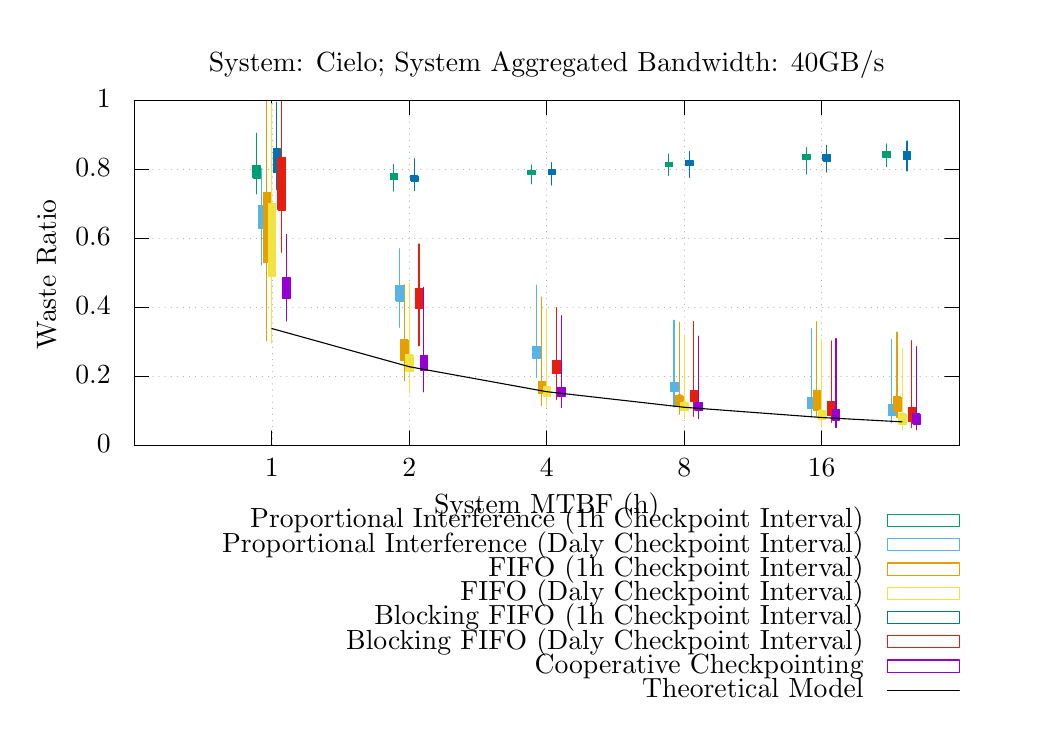
\begin{tikzpicture}[gnuplot]
%% generated with GNUPLOT 5.0p6 (Lua 5.3; terminal rev. 99, script rev. 100)
%% Wed Oct 18 12:29:40 2017
\path (0.000,0.000) rectangle (12.500,8.750);
\gpcolor{color=gp lt color axes}
\gpsetlinetype{gp lt axes}
\gpsetdashtype{gp dt axes}
\gpsetlinewidth{0.50}
\draw[gp path] (1.320,3.449)--(11.793,3.449);
\gpcolor{color=gp lt color border}
\gpsetlinetype{gp lt border}
\gpsetdashtype{gp dt solid}
\gpsetlinewidth{1.00}
\draw[gp path] (1.320,3.449)--(1.500,3.449);
\draw[gp path] (11.793,3.449)--(11.613,3.449);
\node[gp node right] at (1.136,3.449) {$0$};
\gpcolor{color=gp lt color axes}
\gpsetlinetype{gp lt axes}
\gpsetdashtype{gp dt axes}
\gpsetlinewidth{0.50}
\draw[gp path] (1.320,4.324)--(11.793,4.324);
\gpcolor{color=gp lt color border}
\gpsetlinetype{gp lt border}
\gpsetdashtype{gp dt solid}
\gpsetlinewidth{1.00}
\draw[gp path] (1.320,4.324)--(1.500,4.324);
\draw[gp path] (11.793,4.324)--(11.613,4.324);
\node[gp node right] at (1.136,4.324) {$0.2$};
\gpcolor{color=gp lt color axes}
\gpsetlinetype{gp lt axes}
\gpsetdashtype{gp dt axes}
\gpsetlinewidth{0.50}
\draw[gp path] (1.320,5.199)--(11.793,5.199);
\gpcolor{color=gp lt color border}
\gpsetlinetype{gp lt border}
\gpsetdashtype{gp dt solid}
\gpsetlinewidth{1.00}
\draw[gp path] (1.320,5.199)--(1.500,5.199);
\draw[gp path] (11.793,5.199)--(11.613,5.199);
\node[gp node right] at (1.136,5.199) {$0.4$};
\gpcolor{color=gp lt color axes}
\gpsetlinetype{gp lt axes}
\gpsetdashtype{gp dt axes}
\gpsetlinewidth{0.50}
\draw[gp path] (1.320,6.075)--(11.793,6.075);
\gpcolor{color=gp lt color border}
\gpsetlinetype{gp lt border}
\gpsetdashtype{gp dt solid}
\gpsetlinewidth{1.00}
\draw[gp path] (1.320,6.075)--(1.500,6.075);
\draw[gp path] (11.793,6.075)--(11.613,6.075);
\node[gp node right] at (1.136,6.075) {$0.6$};
\gpcolor{color=gp lt color axes}
\gpsetlinetype{gp lt axes}
\gpsetdashtype{gp dt axes}
\gpsetlinewidth{0.50}
\draw[gp path] (1.320,6.950)--(11.793,6.950);
\gpcolor{color=gp lt color border}
\gpsetlinetype{gp lt border}
\gpsetdashtype{gp dt solid}
\gpsetlinewidth{1.00}
\draw[gp path] (1.320,6.950)--(1.500,6.950);
\draw[gp path] (11.793,6.950)--(11.613,6.950);
\node[gp node right] at (1.136,6.950) {$0.8$};
\gpcolor{color=gp lt color axes}
\gpsetlinetype{gp lt axes}
\gpsetdashtype{gp dt axes}
\gpsetlinewidth{0.50}
\draw[gp path] (1.320,7.825)--(11.793,7.825);
\gpcolor{color=gp lt color border}
\gpsetlinetype{gp lt border}
\gpsetdashtype{gp dt solid}
\gpsetlinewidth{1.00}
\draw[gp path] (1.320,7.825)--(1.500,7.825);
\draw[gp path] (11.793,7.825)--(11.613,7.825);
\node[gp node right] at (1.136,7.825) {$1$};
\gpcolor{color=gp lt color axes}
\gpsetlinetype{gp lt axes}
\gpsetdashtype{gp dt axes}
\gpsetlinewidth{0.50}
\draw[gp path] (3.065,3.449)--(3.065,7.825);
\gpcolor{color=gp lt color border}
\gpsetlinetype{gp lt border}
\gpsetdashtype{gp dt solid}
\gpsetlinewidth{1.00}
\draw[gp path] (3.065,3.449)--(3.065,3.629);
\draw[gp path] (3.065,7.825)--(3.065,7.645);
\node[gp node center] at (3.065,3.141) {1};
\gpcolor{color=gp lt color axes}
\gpsetlinetype{gp lt axes}
\gpsetdashtype{gp dt axes}
\gpsetlinewidth{0.50}
\draw[gp path] (4.811,3.449)--(4.811,7.825);
\gpcolor{color=gp lt color border}
\gpsetlinetype{gp lt border}
\gpsetdashtype{gp dt solid}
\gpsetlinewidth{1.00}
\draw[gp path] (4.811,3.449)--(4.811,3.629);
\draw[gp path] (4.811,7.825)--(4.811,7.645);
\node[gp node center] at (4.811,3.141) {2};
\gpcolor{color=gp lt color axes}
\gpsetlinetype{gp lt axes}
\gpsetdashtype{gp dt axes}
\gpsetlinewidth{0.50}
\draw[gp path] (6.556,3.449)--(6.556,7.825);
\gpcolor{color=gp lt color border}
\gpsetlinetype{gp lt border}
\gpsetdashtype{gp dt solid}
\gpsetlinewidth{1.00}
\draw[gp path] (6.556,3.449)--(6.556,3.629);
\draw[gp path] (6.556,7.825)--(6.556,7.645);
\node[gp node center] at (6.556,3.141) {4};
\gpcolor{color=gp lt color axes}
\gpsetlinetype{gp lt axes}
\gpsetdashtype{gp dt axes}
\gpsetlinewidth{0.50}
\draw[gp path] (8.302,3.449)--(8.302,7.825);
\gpcolor{color=gp lt color border}
\gpsetlinetype{gp lt border}
\gpsetdashtype{gp dt solid}
\gpsetlinewidth{1.00}
\draw[gp path] (8.302,3.449)--(8.302,3.629);
\draw[gp path] (8.302,7.825)--(8.302,7.645);
\node[gp node center] at (8.302,3.141) {8};
\gpcolor{color=gp lt color axes}
\gpsetlinetype{gp lt axes}
\gpsetdashtype{gp dt axes}
\gpsetlinewidth{0.50}
\draw[gp path] (10.048,3.449)--(10.048,7.825);
\gpcolor{color=gp lt color border}
\gpsetlinetype{gp lt border}
\gpsetdashtype{gp dt solid}
\gpsetlinewidth{1.00}
\draw[gp path] (10.048,3.449)--(10.048,3.629);
\draw[gp path] (10.048,7.825)--(10.048,7.645);
\node[gp node center] at (10.048,3.141) {16};
\draw[gp path] (1.320,7.825)--(1.320,3.449)--(11.793,3.449)--(11.793,7.825)--cycle;
\node[gp node center,rotate=-270] at (0.246,5.637) {Waste Ratio};
\node[gp node center] at (6.556,2.679) {System MTBF (h)};
\node[gp node center] at (6.556,8.287) {System: Cielo; System Aggregated Bandwidth: 40GB/s};
\node[gp node right] at (10.698,2.490) {Proportional Interference (1h Checkpoint Interval)};
\gpcolor{rgb color={0.000,0.620,0.451}}
\draw[gp path] (10.882,2.413)--(11.798,2.413)--(11.798,2.567)--(10.882,2.567)--cycle;
\gpfill{rgb color={0.000,0.620,0.451}} (2.824,6.846)--(2.914,6.846)--(2.914,7.004)--(2.824,7.004)--cycle;
\draw[gp path] (2.869,6.639)--(2.869,6.846);
\draw[gp path] (2.869,7.004)--(2.869,7.409);
\draw[gp path] (2.824,7.004)--(2.914,7.004)--(2.914,6.846)--(2.824,6.846)--cycle;
\gpfill{rgb color={0.000,0.620,0.451}} (4.570,6.825)--(4.660,6.825)--(4.660,6.894)--(4.570,6.894)--cycle;
\draw[gp path] (4.615,6.675)--(4.615,6.825);
\draw[gp path] (4.615,6.894)--(4.615,7.013);
\draw[gp path] (4.570,6.894)--(4.660,6.894)--(4.660,6.825)--(4.570,6.825)--cycle;
\gpfill{rgb color={0.000,0.620,0.451}} (6.315,6.889)--(6.405,6.889)--(6.405,6.937)--(6.315,6.937)--cycle;
\draw[gp path] (6.360,6.767)--(6.360,6.889);
\draw[gp path] (6.360,6.937)--(6.360,7.007);
\draw[gp path] (6.315,6.937)--(6.405,6.937)--(6.405,6.889)--(6.315,6.889)--cycle;
\gpfill{rgb color={0.000,0.620,0.451}} (8.061,6.990)--(8.151,6.990)--(8.151,7.037)--(8.061,7.037)--cycle;
\draw[gp path] (8.106,6.874)--(8.106,6.990);
\draw[gp path] (8.106,7.037)--(8.106,7.145);
\draw[gp path] (8.061,7.037)--(8.151,7.037)--(8.151,6.990)--(8.061,6.990)--cycle;
\gpfill{rgb color={0.000,0.620,0.451}} (9.806,7.079)--(9.896,7.079)--(9.896,7.140)--(9.806,7.140)--cycle;
\draw[gp path] (9.851,6.891)--(9.851,7.079);
\draw[gp path] (9.851,7.140)--(9.851,7.226);
\draw[gp path] (9.806,7.140)--(9.896,7.140)--(9.896,7.079)--(9.806,7.079)--cycle;
\gpfill{rgb color={0.000,0.620,0.451}} (10.827,7.106)--(10.917,7.106)--(10.917,7.177)--(10.827,7.177)--cycle;
\draw[gp path] (10.872,6.987)--(10.872,7.106);
\draw[gp path] (10.872,7.177)--(10.872,7.273);
\draw[gp path] (10.827,7.177)--(10.917,7.177)--(10.917,7.106)--(10.827,7.106)--cycle;
\gpsetpointsize{0.80}
\gppoint{gp mark 2}{(2.869,6.931)}
\gppoint{gp mark 2}{(4.615,6.859)}
\gppoint{gp mark 2}{(6.360,6.911)}
\gppoint{gp mark 2}{(8.106,7.012)}
\gppoint{gp mark 2}{(9.851,7.106)}
\gppoint{gp mark 2}{(10.872,7.141)}
\gpcolor{color=gp lt color border}
\node[gp node right] at (10.698,2.182) {Proportional Interference (Daly Checkpoint Interval)};
\gpcolor{rgb color={0.337,0.706,0.914}}
\draw[gp path] (10.882,2.105)--(11.798,2.105)--(11.798,2.259)--(10.882,2.259)--cycle;
\gpfill{rgb color={0.337,0.706,0.914}} (2.891,6.207)--(2.981,6.207)--(2.981,6.491)--(2.891,6.491)--cycle;
\draw[gp path] (2.936,5.733)--(2.936,6.207);
\draw[gp path] (2.936,6.491)--(2.936,6.962);
\draw[gp path] (2.891,6.491)--(2.981,6.491)--(2.981,6.207)--(2.891,6.207)--cycle;
\gpfill{rgb color={0.337,0.706,0.914}} (4.637,5.280)--(4.727,5.280)--(4.727,5.478)--(4.637,5.478)--cycle;
\draw[gp path] (4.682,4.945)--(4.682,5.280);
\draw[gp path] (4.682,5.478)--(4.682,5.943);
\draw[gp path] (4.637,5.478)--(4.727,5.478)--(4.727,5.280)--(4.637,5.280)--cycle;
\gpfill{rgb color={0.337,0.706,0.914}} (6.382,4.551)--(6.472,4.551)--(6.472,4.702)--(6.382,4.702)--cycle;
\draw[gp path] (6.427,4.305)--(6.427,4.551);
\draw[gp path] (6.427,4.702)--(6.427,5.480);
\draw[gp path] (6.382,4.702)--(6.472,4.702)--(6.472,4.551)--(6.382,4.551)--cycle;
\gpfill{rgb color={0.337,0.706,0.914}} (8.128,4.132)--(8.218,4.132)--(8.218,4.248)--(8.128,4.248)--cycle;
\draw[gp path] (8.173,3.934)--(8.173,4.132);
\draw[gp path] (8.173,4.248)--(8.173,5.034);
\draw[gp path] (8.128,4.248)--(8.218,4.248)--(8.218,4.132)--(8.128,4.132)--cycle;
\gpfill{rgb color={0.337,0.706,0.914}} (9.873,3.914)--(9.963,3.914)--(9.963,4.048)--(9.873,4.048)--cycle;
\draw[gp path] (9.918,3.807)--(9.918,3.914);
\draw[gp path] (9.918,4.048)--(9.918,4.927);
\draw[gp path] (9.873,4.048)--(9.963,4.048)--(9.963,3.914)--(9.873,3.914)--cycle;
\gpfill{rgb color={0.337,0.706,0.914}} (10.894,3.829)--(10.984,3.829)--(10.984,3.961)--(10.894,3.961)--cycle;
\draw[gp path] (10.939,3.731)--(10.939,3.829);
\draw[gp path] (10.939,3.961)--(10.939,4.791);
\draw[gp path] (10.894,3.961)--(10.984,3.961)--(10.984,3.829)--(10.894,3.829)--cycle;
\gppoint{gp mark 3}{(2.936,6.355)}
\gppoint{gp mark 3}{(4.682,5.380)}
\gppoint{gp mark 3}{(6.427,4.648)}
\gppoint{gp mark 3}{(8.173,4.222)}
\gppoint{gp mark 3}{(9.918,4.017)}
\gppoint{gp mark 3}{(10.939,3.939)}
\gpcolor{color=gp lt color border}
\node[gp node right] at (10.698,1.874) {FIFO (1h Checkpoint Interval)};
\gpcolor{rgb color={0.902,0.624,0.000}}
\draw[gp path] (10.882,1.797)--(11.798,1.797)--(11.798,1.951)--(10.882,1.951)--cycle;
\gpfill{rgb color={0.902,0.624,0.000}} (2.957,5.767)--(3.047,5.767)--(3.047,6.655)--(2.957,6.655)--cycle;
\draw[gp path] (3.002,4.772)--(3.002,5.767);
\draw[gp path] (3.002,6.655)--(3.002,7.825);
\draw[gp path] (2.957,6.655)--(3.047,6.655)--(3.047,5.767)--(2.957,5.767)--cycle;
\gpfill{rgb color={0.902,0.624,0.000}} (4.702,4.525)--(4.792,4.525)--(4.792,4.785)--(4.702,4.785)--cycle;
\draw[gp path] (4.747,4.264)--(4.747,4.525);
\draw[gp path] (4.747,4.785)--(4.747,5.485);
\draw[gp path] (4.702,4.785)--(4.792,4.785)--(4.792,4.525)--(4.702,4.525)--cycle;
\gpfill{rgb color={0.902,0.624,0.000}} (6.448,4.104)--(6.538,4.104)--(6.538,4.253)--(6.448,4.253)--cycle;
\draw[gp path] (6.493,3.950)--(6.493,4.104);
\draw[gp path] (6.493,4.253)--(6.493,5.329);
\draw[gp path] (6.448,4.253)--(6.538,4.253)--(6.538,4.104)--(6.448,4.104)--cycle;
\gpfill{rgb color={0.902,0.624,0.000}} (8.193,3.951)--(8.283,3.951)--(8.283,4.073)--(8.193,4.073)--cycle;
\draw[gp path] (8.238,3.839)--(8.238,3.951);
\draw[gp path] (8.238,4.073)--(8.238,5.011);
\draw[gp path] (8.193,4.073)--(8.283,4.073)--(8.283,3.951)--(8.193,3.951)--cycle;
\gpfill{rgb color={0.902,0.624,0.000}} (9.939,3.891)--(10.029,3.891)--(10.029,4.137)--(9.939,4.137)--cycle;
\draw[gp path] (9.984,3.813)--(9.984,3.891);
\draw[gp path] (9.984,4.137)--(9.984,5.015);
\draw[gp path] (9.939,4.137)--(10.029,4.137)--(10.029,3.891)--(9.939,3.891)--cycle;
\gpfill{rgb color={0.902,0.624,0.000}} (10.960,3.875)--(11.050,3.875)--(11.050,4.060)--(10.960,4.060)--cycle;
\draw[gp path] (11.005,3.799)--(11.005,3.875);
\draw[gp path] (11.005,4.060)--(11.005,4.883);
\draw[gp path] (10.960,4.060)--(11.050,4.060)--(11.050,3.875)--(10.960,3.875)--cycle;
\gppoint{gp mark 4}{(3.002,6.245)}
\gppoint{gp mark 4}{(4.747,4.675)}
\gppoint{gp mark 4}{(6.493,4.225)}
\gppoint{gp mark 4}{(8.238,4.080)}
\gppoint{gp mark 4}{(9.984,4.055)}
\gppoint{gp mark 4}{(11.005,4.015)}
\gpcolor{color=gp lt color border}
\node[gp node right] at (10.698,1.566) {FIFO (Daly Checkpoint Interval)};
\gpcolor{rgb color={0.941,0.894,0.259}}
\draw[gp path] (10.882,1.489)--(11.798,1.489)--(11.798,1.643)--(10.882,1.643)--cycle;
\gpfill{rgb color={0.941,0.894,0.259}} (3.020,5.597)--(3.110,5.597)--(3.110,6.515)--(3.020,6.515)--cycle;
\draw[gp path] (3.065,4.744)--(3.065,5.597);
\draw[gp path] (3.065,6.515)--(3.065,7.784);
\draw[gp path] (3.020,6.515)--(3.110,6.515)--(3.110,5.597)--(3.020,5.597)--cycle;
\gpfill{rgb color={0.941,0.894,0.259}} (4.766,4.392)--(4.856,4.392)--(4.856,4.598)--(4.766,4.598)--cycle;
\draw[gp path] (4.811,4.108)--(4.811,4.392);
\draw[gp path] (4.811,4.598)--(4.811,5.501);
\draw[gp path] (4.766,4.598)--(4.856,4.598)--(4.856,4.392)--(4.766,4.392)--cycle;
\gpfill{rgb color={0.941,0.894,0.259}} (6.511,4.067)--(6.601,4.067)--(6.601,4.190)--(6.511,4.190)--cycle;
\draw[gp path] (6.556,3.937)--(6.556,4.067);
\draw[gp path] (6.556,4.190)--(6.556,5.184);
\draw[gp path] (6.511,4.190)--(6.601,4.190)--(6.601,4.067)--(6.511,4.067)--cycle;
\gpfill{rgb color={0.941,0.894,0.259}} (8.257,3.893)--(8.347,3.893)--(8.347,3.989)--(8.257,3.989)--cycle;
\draw[gp path] (8.302,3.786)--(8.302,3.893);
\draw[gp path] (8.302,3.989)--(8.302,4.843);
\draw[gp path] (8.257,3.989)--(8.347,3.989)--(8.347,3.893)--(8.257,3.893)--cycle;
\gpfill{rgb color={0.941,0.894,0.259}} (10.003,3.775)--(10.093,3.775)--(10.093,3.893)--(10.003,3.893)--cycle;
\draw[gp path] (10.048,3.679)--(10.048,3.775);
\draw[gp path] (10.048,3.893)--(10.048,4.792);
\draw[gp path] (10.003,3.893)--(10.093,3.893)--(10.093,3.775)--(10.003,3.775)--cycle;
\gpfill{rgb color={0.941,0.894,0.259}} (11.024,3.720)--(11.114,3.720)--(11.114,3.845)--(11.024,3.845)--cycle;
\draw[gp path] (11.069,3.641)--(11.069,3.720);
\draw[gp path] (11.069,3.845)--(11.069,4.675);
\draw[gp path] (11.024,3.845)--(11.114,3.845)--(11.114,3.720)--(11.024,3.720)--cycle;
\gppoint{gp mark 5}{(3.065,6.077)}
\gppoint{gp mark 5}{(4.811,4.519)}
\gppoint{gp mark 5}{(6.556,4.174)}
\gppoint{gp mark 5}{(8.302,3.991)}
\gppoint{gp mark 5}{(10.048,3.885)}
\gppoint{gp mark 5}{(11.069,3.837)}
\gpcolor{color=gp lt color border}
\node[gp node right] at (10.698,1.258) {Blocking FIFO (1h Checkpoint Interval)};
\gpcolor{rgb color={0.000,0.447,0.698}}
\draw[gp path] (10.882,1.181)--(11.798,1.181)--(11.798,1.335)--(10.882,1.335)--cycle;
\gpfill{rgb color={0.000,0.447,0.698}} (3.083,6.912)--(3.173,6.912)--(3.173,7.210)--(3.083,7.210)--cycle;
\draw[gp path] (3.128,6.691)--(3.128,6.912);
\draw[gp path] (3.128,7.210)--(3.128,7.803);
\draw[gp path] (3.083,7.210)--(3.173,7.210)--(3.173,6.912)--(3.083,6.912)--cycle;
\gpfill{rgb color={0.000,0.447,0.698}} (4.828,6.807)--(4.918,6.807)--(4.918,6.870)--(4.828,6.870)--cycle;
\draw[gp path] (4.873,6.681)--(4.873,6.807);
\draw[gp path] (4.873,6.870)--(4.873,7.085);
\draw[gp path] (4.828,6.870)--(4.918,6.870)--(4.918,6.807)--(4.828,6.807)--cycle;
\gpfill{rgb color={0.000,0.447,0.698}} (6.574,6.896)--(6.664,6.896)--(6.664,6.943)--(6.574,6.943)--cycle;
\draw[gp path] (6.619,6.750)--(6.619,6.896);
\draw[gp path] (6.619,6.943)--(6.619,7.035);
\draw[gp path] (6.574,6.943)--(6.664,6.943)--(6.664,6.896)--(6.574,6.896)--cycle;
\gpfill{rgb color={0.000,0.447,0.698}} (8.319,7.000)--(8.409,7.000)--(8.409,7.067)--(8.319,7.067)--cycle;
\draw[gp path] (8.364,6.848)--(8.364,7.000);
\draw[gp path] (8.364,7.067)--(8.364,7.177);
\draw[gp path] (8.319,7.067)--(8.409,7.067)--(8.409,7.000)--(8.319,7.000)--cycle;
\gpfill{rgb color={0.000,0.447,0.698}} (10.065,7.060)--(10.155,7.060)--(10.155,7.138)--(10.065,7.138)--cycle;
\draw[gp path] (10.110,6.915)--(10.110,7.060);
\draw[gp path] (10.110,7.138)--(10.110,7.256);
\draw[gp path] (10.065,7.138)--(10.155,7.138)--(10.155,7.060)--(10.065,7.060)--cycle;
\gpfill{rgb color={0.000,0.447,0.698}} (11.086,7.079)--(11.176,7.079)--(11.176,7.174)--(11.086,7.174)--cycle;
\draw[gp path] (11.131,6.931)--(11.131,7.079);
\draw[gp path] (11.131,7.174)--(11.131,7.309);
\draw[gp path] (11.086,7.174)--(11.176,7.174)--(11.176,7.079)--(11.086,7.079)--cycle;
\gppoint{gp mark 6}{(3.128,7.093)}
\gppoint{gp mark 6}{(4.873,6.841)}
\gppoint{gp mark 6}{(6.619,6.919)}
\gppoint{gp mark 6}{(8.364,7.032)}
\gppoint{gp mark 6}{(10.110,7.099)}
\gppoint{gp mark 6}{(11.131,7.126)}
\gpcolor{color=gp lt color border}
\node[gp node right] at (10.698,0.950) {Blocking FIFO (Daly Checkpoint Interval)};
\gpcolor{rgb color={0.898,0.118,0.063}}
\draw[gp path] (10.882,0.873)--(11.798,0.873)--(11.798,1.027)--(10.882,1.027)--cycle;
\gpfill{rgb color={0.898,0.118,0.063}} (3.143,6.440)--(3.233,6.440)--(3.233,7.103)--(3.143,7.103)--cycle;
\draw[gp path] (3.188,5.896)--(3.188,6.440);
\draw[gp path] (3.188,7.103)--(3.188,7.824);
\draw[gp path] (3.143,7.103)--(3.233,7.103)--(3.233,6.440)--(3.143,6.440)--cycle;
\gpfill{rgb color={0.898,0.118,0.063}} (4.889,5.193)--(4.979,5.193)--(4.979,5.443)--(4.889,5.443)--cycle;
\draw[gp path] (4.934,4.709)--(4.934,5.193);
\draw[gp path] (4.934,5.443)--(4.934,6.003);
\draw[gp path] (4.889,5.443)--(4.979,5.443)--(4.979,5.193)--(4.889,5.193)--cycle;
\gpfill{rgb color={0.898,0.118,0.063}} (6.634,4.360)--(6.724,4.360)--(6.724,4.526)--(6.634,4.526)--cycle;
\draw[gp path] (6.679,4.025)--(6.679,4.360);
\draw[gp path] (6.679,4.526)--(6.679,5.193);
\draw[gp path] (6.634,4.526)--(6.724,4.526)--(6.724,4.360)--(6.634,4.360)--cycle;
\gpfill{rgb color={0.898,0.118,0.063}} (8.380,4.006)--(8.470,4.006)--(8.470,4.136)--(8.380,4.136)--cycle;
\draw[gp path] (8.425,3.814)--(8.425,4.006);
\draw[gp path] (8.425,4.136)--(8.425,5.018);
\draw[gp path] (8.380,4.136)--(8.470,4.136)--(8.470,4.006)--(8.380,4.006)--cycle;
\gpfill{rgb color={0.898,0.118,0.063}} (10.125,3.826)--(10.215,3.826)--(10.215,4.002)--(10.125,4.002)--cycle;
\draw[gp path] (10.170,3.739)--(10.170,3.826);
\draw[gp path] (10.170,4.002)--(10.170,4.772);
\draw[gp path] (10.125,4.002)--(10.215,4.002)--(10.215,3.826)--(10.125,3.826)--cycle;
\gpfill{rgb color={0.898,0.118,0.063}} (11.146,3.756)--(11.236,3.756)--(11.236,3.925)--(11.146,3.925)--cycle;
\draw[gp path] (11.191,3.671)--(11.191,3.756);
\draw[gp path] (11.191,3.925)--(11.191,4.774);
\draw[gp path] (11.146,3.925)--(11.236,3.925)--(11.236,3.756)--(11.146,3.756)--cycle;
\gppoint{gp mark 7}{(3.188,6.792)}
\gppoint{gp mark 7}{(4.934,5.324)}
\gppoint{gp mark 7}{(6.679,4.465)}
\gppoint{gp mark 7}{(8.425,4.114)}
\gppoint{gp mark 7}{(10.170,3.955)}
\gppoint{gp mark 7}{(11.191,3.885)}
\gpcolor{color=gp lt color border}
\node[gp node right] at (10.698,0.642) {Cooperative Checkpointing};
\gpcolor{rgb color={0.580,0.000,0.827}}
\draw[gp path] (10.882,0.565)--(11.798,0.565)--(11.798,0.719)--(10.882,0.719)--cycle;
\gpfill{rgb color={0.580,0.000,0.827}} (3.203,5.312)--(3.293,5.312)--(3.293,5.579)--(3.203,5.579)--cycle;
\draw[gp path] (3.248,5.025)--(3.248,5.312);
\draw[gp path] (3.248,5.579)--(3.248,6.125);
\draw[gp path] (3.203,5.579)--(3.293,5.579)--(3.293,5.312)--(3.203,5.312)--cycle;
\gpfill{rgb color={0.580,0.000,0.827}} (4.948,4.408)--(5.038,4.408)--(5.038,4.586)--(4.948,4.586)--cycle;
\draw[gp path] (4.993,4.124)--(4.993,4.408);
\draw[gp path] (4.993,4.586)--(4.993,5.452);
\draw[gp path] (4.948,4.586)--(5.038,4.586)--(5.038,4.408)--(4.948,4.408)--cycle;
\gpfill{rgb color={0.580,0.000,0.827}} (6.694,4.067)--(6.784,4.067)--(6.784,4.185)--(6.694,4.185)--cycle;
\draw[gp path] (6.739,3.925)--(6.739,4.067);
\draw[gp path] (6.739,4.185)--(6.739,5.093);
\draw[gp path] (6.694,4.185)--(6.784,4.185)--(6.784,4.067)--(6.694,4.067)--cycle;
\gpfill{rgb color={0.580,0.000,0.827}} (8.439,3.895)--(8.529,3.895)--(8.529,3.987)--(8.439,3.987)--cycle;
\draw[gp path] (8.484,3.785)--(8.484,3.895);
\draw[gp path] (8.484,3.987)--(8.484,4.832);
\draw[gp path] (8.439,3.987)--(8.529,3.987)--(8.529,3.895)--(8.439,3.895)--cycle;
\gpfill{rgb color={0.580,0.000,0.827}} (10.185,3.773)--(10.275,3.773)--(10.275,3.897)--(10.185,3.897)--cycle;
\draw[gp path] (10.230,3.672)--(10.230,3.773);
\draw[gp path] (10.230,3.897)--(10.230,4.801);
\draw[gp path] (10.185,3.897)--(10.275,3.897)--(10.275,3.773)--(10.185,3.773)--cycle;
\gpfill{rgb color={0.580,0.000,0.827}} (11.206,3.722)--(11.296,3.722)--(11.296,3.846)--(11.206,3.846)--cycle;
\draw[gp path] (11.251,3.642)--(11.251,3.722);
\draw[gp path] (11.251,3.846)--(11.251,4.698);
\draw[gp path] (11.206,3.846)--(11.296,3.846)--(11.296,3.722)--(11.206,3.722)--cycle;
\gppoint{gp mark 1}{(3.248,5.451)}
\gppoint{gp mark 1}{(4.993,4.518)}
\gppoint{gp mark 1}{(6.739,4.173)}
\gppoint{gp mark 1}{(8.484,3.992)}
\gppoint{gp mark 1}{(10.230,3.884)}
\gppoint{gp mark 1}{(11.251,3.836)}
\gpcolor{color=gp lt color border}
\node[gp node right] at (10.698,0.334) {Theoretical Model};
\gpcolor{rgb color={0.000,0.000,0.000}}
\draw[gp path] (10.882,0.334)--(11.798,0.334);
\draw[gp path] (3.065,4.929)--(4.811,4.444)--(6.556,4.127)--(8.302,3.929)--(10.048,3.799)%
  --(11.069,3.744);
\gpcolor{color=gp lt color border}
\draw[gp path] (1.320,7.825)--(1.320,3.449)--(11.793,3.449)--(11.793,7.825)--cycle;
%% coordinates of the plot area
\gpdefrectangularnode{gp plot 1}{\pgfpoint{1.320cm}{3.449cm}}{\pgfpoint{11.793cm}{7.825cm}}
\end{tikzpicture}
%% gnuplot variables
}
    
    $\bandavail=40 \text{GBs}$
  \end{center}
 
       \end{frame}

    
      \begin{frame}
  \frametitle{Prospective system (1/2)}
 
 \begin{itemize}
\item Aurora-like\\
7PB of main memory and 50,000 compute nodes 
\item Scale APEX workflow\\
accordingly to Aurora/Celio memory size increase 

\end{itemize}

 
       \end{frame}
       
      \begin{frame}
       \frametitle{Prospective system (2/2)}


 
  \begin{center}
    \resizebox{0.95\linewidth}{!}{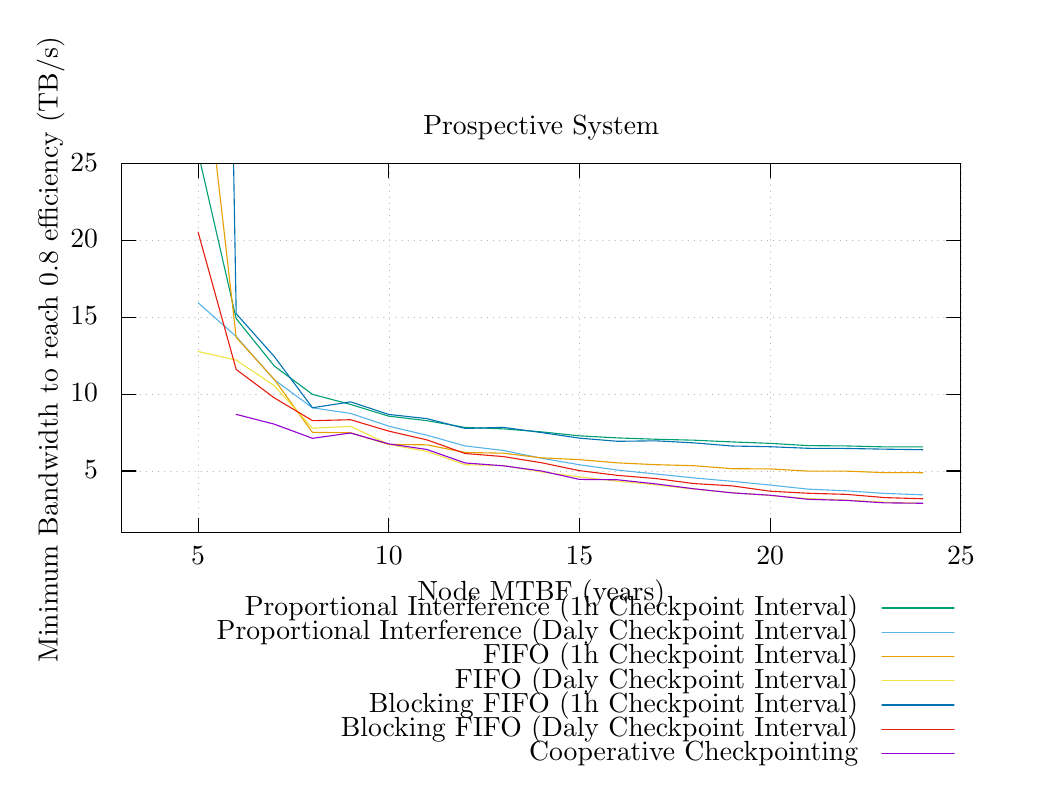
\begin{tikzpicture}[gnuplot]
%% generated with GNUPLOT 5.0p6 (Lua 5.3; terminal rev. 99, script rev. 100)
%% Wed Oct 18 12:29:10 2017
\path (0.000,0.000) rectangle (12.500,8.750);
\gpcolor{color=gp lt color axes}
\gpsetlinetype{gp lt axes}
\gpsetdashtype{gp dt axes}
\gpsetlinewidth{0.50}
\draw[gp path] (1.136,3.922)--(11.793,3.922);
\gpcolor{color=gp lt color border}
\gpsetlinetype{gp lt border}
\gpsetdashtype{gp dt solid}
\gpsetlinewidth{1.00}
\draw[gp path] (1.136,3.922)--(1.316,3.922);
\draw[gp path] (11.793,3.922)--(11.613,3.922);
\node[gp node right] at (0.952,3.922) {$5$};
\gpcolor{color=gp lt color axes}
\gpsetlinetype{gp lt axes}
\gpsetdashtype{gp dt axes}
\gpsetlinewidth{0.50}
\draw[gp path] (1.136,4.898)--(11.793,4.898);
\gpcolor{color=gp lt color border}
\gpsetlinetype{gp lt border}
\gpsetdashtype{gp dt solid}
\gpsetlinewidth{1.00}
\draw[gp path] (1.136,4.898)--(1.316,4.898);
\draw[gp path] (11.793,4.898)--(11.613,4.898);
\node[gp node right] at (0.952,4.898) {$10$};
\gpcolor{color=gp lt color axes}
\gpsetlinetype{gp lt axes}
\gpsetdashtype{gp dt axes}
\gpsetlinewidth{0.50}
\draw[gp path] (1.136,5.873)--(11.793,5.873);
\gpcolor{color=gp lt color border}
\gpsetlinetype{gp lt border}
\gpsetdashtype{gp dt solid}
\gpsetlinewidth{1.00}
\draw[gp path] (1.136,5.873)--(1.316,5.873);
\draw[gp path] (11.793,5.873)--(11.613,5.873);
\node[gp node right] at (0.952,5.873) {$15$};
\gpcolor{color=gp lt color axes}
\gpsetlinetype{gp lt axes}
\gpsetdashtype{gp dt axes}
\gpsetlinewidth{0.50}
\draw[gp path] (1.136,6.849)--(11.793,6.849);
\gpcolor{color=gp lt color border}
\gpsetlinetype{gp lt border}
\gpsetdashtype{gp dt solid}
\gpsetlinewidth{1.00}
\draw[gp path] (1.136,6.849)--(1.316,6.849);
\draw[gp path] (11.793,6.849)--(11.613,6.849);
\node[gp node right] at (0.952,6.849) {$20$};
\gpcolor{color=gp lt color axes}
\gpsetlinetype{gp lt axes}
\gpsetdashtype{gp dt axes}
\gpsetlinewidth{0.50}
\draw[gp path] (1.136,7.825)--(11.793,7.825);
\gpcolor{color=gp lt color border}
\gpsetlinetype{gp lt border}
\gpsetdashtype{gp dt solid}
\gpsetlinewidth{1.00}
\draw[gp path] (1.136,7.825)--(1.316,7.825);
\draw[gp path] (11.793,7.825)--(11.613,7.825);
\node[gp node right] at (0.952,7.825) {$25$};
\gpcolor{color=gp lt color axes}
\gpsetlinetype{gp lt axes}
\gpsetdashtype{gp dt axes}
\gpsetlinewidth{0.50}
\draw[gp path] (2.105,3.141)--(2.105,7.825);
\gpcolor{color=gp lt color border}
\gpsetlinetype{gp lt border}
\gpsetdashtype{gp dt solid}
\gpsetlinewidth{1.00}
\draw[gp path] (2.105,3.141)--(2.105,3.321);
\draw[gp path] (2.105,7.825)--(2.105,7.645);
\node[gp node center] at (2.105,2.833) {$5$};
\gpcolor{color=gp lt color axes}
\gpsetlinetype{gp lt axes}
\gpsetdashtype{gp dt axes}
\gpsetlinewidth{0.50}
\draw[gp path] (4.527,3.141)--(4.527,7.825);
\gpcolor{color=gp lt color border}
\gpsetlinetype{gp lt border}
\gpsetdashtype{gp dt solid}
\gpsetlinewidth{1.00}
\draw[gp path] (4.527,3.141)--(4.527,3.321);
\draw[gp path] (4.527,7.825)--(4.527,7.645);
\node[gp node center] at (4.527,2.833) {$10$};
\gpcolor{color=gp lt color axes}
\gpsetlinetype{gp lt axes}
\gpsetdashtype{gp dt axes}
\gpsetlinewidth{0.50}
\draw[gp path] (6.949,3.141)--(6.949,7.825);
\gpcolor{color=gp lt color border}
\gpsetlinetype{gp lt border}
\gpsetdashtype{gp dt solid}
\gpsetlinewidth{1.00}
\draw[gp path] (6.949,3.141)--(6.949,3.321);
\draw[gp path] (6.949,7.825)--(6.949,7.645);
\node[gp node center] at (6.949,2.833) {$15$};
\gpcolor{color=gp lt color axes}
\gpsetlinetype{gp lt axes}
\gpsetdashtype{gp dt axes}
\gpsetlinewidth{0.50}
\draw[gp path] (9.371,3.141)--(9.371,7.825);
\gpcolor{color=gp lt color border}
\gpsetlinetype{gp lt border}
\gpsetdashtype{gp dt solid}
\gpsetlinewidth{1.00}
\draw[gp path] (9.371,3.141)--(9.371,3.321);
\draw[gp path] (9.371,7.825)--(9.371,7.645);
\node[gp node center] at (9.371,2.833) {$20$};
\gpcolor{color=gp lt color axes}
\gpsetlinetype{gp lt axes}
\gpsetdashtype{gp dt axes}
\gpsetlinewidth{0.50}
\draw[gp path] (11.793,3.141)--(11.793,7.825);
\gpcolor{color=gp lt color border}
\gpsetlinetype{gp lt border}
\gpsetdashtype{gp dt solid}
\gpsetlinewidth{1.00}
\draw[gp path] (11.793,3.141)--(11.793,3.321);
\draw[gp path] (11.793,7.825)--(11.793,7.645);
\node[gp node center] at (11.793,2.833) {$25$};
\draw[gp path] (1.136,7.825)--(1.136,3.141)--(11.793,3.141)--(11.793,7.825)--cycle;
\node[gp node center,rotate=-270] at (0.246,5.483) {Minimum Bandwidth to reach 0.8 efficiency (TB/s)};
\node[gp node center] at (6.464,2.371) {Node MTBF (years)};
\node[gp node center] at (6.464,8.287) {Prospective System};
\node[gp node right] at (10.606,2.182) {Proportional Interference (1h Checkpoint Interval)};
\gpcolor{rgb color={0.000,0.620,0.451}}
\draw[gp path] (10.790,2.182)--(11.706,2.182);
\draw[gp path] (2.138,7.825)--(2.589,5.857)--(3.074,5.254)--(3.558,4.895)--(4.042,4.767)%
  --(4.527,4.618)--(5.011,4.561)--(5.496,4.475)--(5.980,4.457)--(6.465,4.419)--(6.949,4.368)%
  --(7.433,4.342)--(7.918,4.325)--(8.402,4.313)--(8.887,4.291)--(9.371,4.273)--(9.855,4.244)%
  --(10.340,4.240)--(10.824,4.228)--(11.309,4.228);
\gpcolor{color=gp lt color border}
\node[gp node right] at (10.606,1.874) {Proportional Interference (Daly Checkpoint Interval)};
\gpcolor{rgb color={0.337,0.706,0.914}}
\draw[gp path] (10.790,1.874)--(11.706,1.874);
\draw[gp path] (2.105,6.059)--(2.589,5.630)--(3.074,5.080)--(3.558,4.724)--(4.042,4.653)%
  --(4.527,4.491)--(5.011,4.376)--(5.496,4.240)--(5.980,4.183)--(6.465,4.084)--(6.949,4.001)%
  --(7.433,3.933)--(7.918,3.884)--(8.402,3.834)--(8.887,3.791)--(9.371,3.743)--(9.855,3.691)%
  --(10.340,3.670)--(10.824,3.637)--(11.309,3.619);
\gpcolor{color=gp lt color border}
\node[gp node right] at (10.606,1.566) {FIFO (1h Checkpoint Interval)};
\gpcolor{rgb color={0.902,0.624,0.000}}
\draw[gp path] (10.790,1.566)--(11.706,1.566);
\draw[gp path] (2.337,7.825)--(2.589,5.619)--(3.074,5.083)--(3.558,4.412)--(4.042,4.407)%
  --(4.527,4.259)--(5.011,4.254)--(5.496,4.157)--(5.980,4.148)--(6.465,4.089)--(6.949,4.066)%
  --(7.433,4.025)--(7.918,4.002)--(8.402,3.989)--(8.887,3.951)--(9.371,3.948)--(9.855,3.920)%
  --(10.340,3.920)--(10.824,3.901)--(11.309,3.900);
\gpcolor{color=gp lt color border}
\node[gp node right] at (10.606,1.258) {FIFO (Daly Checkpoint Interval)};
\gpcolor{rgb color={0.941,0.894,0.259}}
\draw[gp path] (10.790,1.258)--(11.706,1.258);
\draw[gp path] (2.105,5.440)--(2.589,5.330)--(3.074,5.005)--(3.558,4.466)--(4.042,4.489)%
  --(4.527,4.260)--(5.011,4.170)--(5.496,4.002)--(5.980,3.991)--(6.465,3.910)--(6.949,3.847)%
  --(7.433,3.792)--(7.918,3.747)--(8.402,3.691)--(8.887,3.646)--(9.371,3.610)--(9.855,3.572)%
  --(10.340,3.553)--(10.824,3.526)--(11.309,3.510);
\gpcolor{color=gp lt color border}
\node[gp node right] at (10.606,0.950) {Blocking FIFO (1h Checkpoint Interval)};
\gpcolor{rgb color={0.000,0.447,0.698}}
\draw[gp path] (10.790,0.950)--(11.706,0.950);
\draw[gp path] (2.556,7.825)--(2.589,5.919)--(3.074,5.374)--(3.558,4.725)--(4.042,4.800)%
  --(4.527,4.640)--(5.011,4.587)--(5.496,4.462)--(5.980,4.476)--(6.465,4.410)--(6.949,4.339)%
  --(7.433,4.299)--(7.918,4.305)--(8.402,4.279)--(8.887,4.239)--(9.371,4.230)--(9.855,4.210)%
  --(10.340,4.208)--(10.824,4.199)--(11.309,4.192);
\gpcolor{color=gp lt color border}
\node[gp node right] at (10.606,0.642) {Blocking FIFO (Daly Checkpoint Interval)};
\gpcolor{rgb color={0.898,0.118,0.063}}
\draw[gp path] (10.790,0.642)--(11.706,0.642);
\draw[gp path] (2.105,6.956)--(2.589,5.211)--(3.074,4.850)--(3.558,4.561)--(4.042,4.573)%
  --(4.527,4.428)--(5.011,4.317)--(5.496,4.144)--(5.980,4.105)--(6.465,4.027)--(6.949,3.926)%
  --(7.433,3.866)--(7.918,3.826)--(8.402,3.762)--(8.887,3.733)--(9.371,3.665)--(9.855,3.639)%
  --(10.340,3.625)--(10.824,3.584)--(11.309,3.569);
\gpcolor{color=gp lt color border}
\node[gp node right] at (10.606,0.334) {Cooperative Checkpointing};
\gpcolor{rgb color={0.580,0.000,0.827}}
\draw[gp path] (10.790,0.334)--(11.706,0.334);
\draw[gp path] (2.589,4.641)--(3.074,4.516)--(3.558,4.337)--(4.042,4.404)--(4.527,4.266)%
  --(5.011,4.195)--(5.496,4.024)--(5.980,3.988)--(6.465,3.922)--(6.949,3.815)--(7.433,3.810)%
  --(7.918,3.758)--(8.402,3.696)--(8.887,3.644)--(9.371,3.614)--(9.855,3.562)--(10.340,3.548)%
  --(10.824,3.517)--(11.309,3.512);
\gpcolor{color=gp lt color border}
\draw[gp path] (1.136,7.825)--(1.136,3.141)--(11.793,3.141)--(11.793,7.825)--cycle;
%% coordinates of the plot area
\gpdefrectangularnode{gp plot 1}{\pgfpoint{1.136cm}{3.141cm}}{\pgfpoint{11.793cm}{7.825cm}}
\end{tikzpicture}
%% gnuplot variables
}
  \end{center}
 
 \vfill
    \centerline{Minimum aggregated filesystem bandwidth to reach 80\%
    efficiency}

       \end{frame}
       
     

\section{Conclusion}

     \begin{frame}
  \frametitle{Conclusion}

\begin{itemize}
\item High pressure on stable storage $\Rightarrow$ \redd{I/O contention}
\item Comprehensive I/O interference model
\item Multiple I/O scheduling algorithms 
\item Improving platform job throughput via waste minimization
\item Show a path to supporting C/R on prospective
system\\
while maintaining a 80\% platform efficiency
\item \green{Future work}: burst buffers and NVRAM
\end{itemize}

  \end{frame}

%\section*{Backup Slides}



\end{document}
